

\begin{table*}
  %\vspace{-0.2in}
  \centering
\begin{threeparttable}
  \caption{Implementations and Parameter Settings of the Considered Baselines}\label{table:baselines}
\begin{tabular}{llclc}\toprule
  \multicolumn{1}{c}{\textbf{Algorithm}}          &
  \multicolumn{1}{c}{\textbf{Classification}}     &
  \multicolumn{1}{c}{\textbf{Implementation}}     &
  \multicolumn{1}{c}{\textbf{Parameter Settings}} &
  \multicolumn{1}{c}{\textbf{Reference}} \\\midrule
  OSRAD  & Diffusion       & Custom            & \(W_{\text{kuan}}= 5 \times 5\), \(c_{\text{tang}} = 0.1\), \(N_{\text{iteration}}=30\), \(\Delta t = 1\) & \cite{krissian_oriented_2007}  \\
  ADMSS  & Diffusion       & Official\tnote{1} & \(N_{\text{class}} = 4\), \(N_{\text{memory}}=5\), \(N_{\text{iteration}} = 20\), \(\sigma = 0.1\), \(\rho = 0.1\)  & \cite{ramos-llorden_anisotropic_2015} \\
  LPNDSF & Diffusion       & Custom            & \(r = [0.1, 1.0, 0.1]\), \(k = [0.3, 0.1, 0.1]\) & \cite{zhang_multiscale_2006} \\
  MNLM   & Non-local mean  & Custom            & \(M = 19 \times 19\), \(K = 3 \times 3\), \(I = 5\), \(h=0.1\) & \cite{breivik_realtime_2017} \\
  NLLR   & Non-local mean \& Low-rank recon.   & Official\tnote{2} & \(H = 10\), \(\beta = 10\) & \cite{zhu_nonlocal_2017} \\
  PFDTV  & Diffusion \& TV regularization    & Custom\tnote{3}   & \(N_{\text{iteration}} = 10\), \(s=15\) & \cite{mei_phase_2020} \\
  \bottomrule
\end{tabular}
\begin{tablenotes}
  \item[1] \url{https://www.mathworks.com/matlabcentral/fileexchange/52988-anisotropic-diffusion-with-memory-based-on-speckle-statistics-for-ultrasound-images}
  \item[2] \url{https://appsrv.cse.cuhk.edu.hk/~lzhu/webpage_despeckling_cvpr2017/index.html}
  \item[3] Based on the official implementation available at \url{https://github.com/Binjie-Qin/PFDTV}.
\end{tablenotes}
\end{threeparttable}
\vspace{-0.1in}
\end{table*}

%%% Local Variables:
%%% TeX-master: "master"
%%% End:

%

\section{Experiments}\label{section:eval}
%% We evaluate the USDG by tuning the parameters of the CLPD.
%% Practicing sonographers were asked to tune the CLPD on \textit{in vivo} images.
%% We analyze the resulting CLPD configurations and compare them against multiple baseline image enhancement algrotithms.
%The experimental setup and protocols are described in~\cref{section:experiment_design}, while the ultrasound image data are discussed in~\cref{section:data}.
%The baseline image enhancement algorithms to be compared against the CLPD are discussed in~\cref{section:baseline}.

\subsection{Experimental Setup}
\subsubsection{Experiment Design}\label{section:experiment_design}
%\paragraph{Sonographer Subjects}
We recruited five sonographers and a cardiologist (also referred to as ``a sonographer'') from the Kangbuk Samsung Hospital Total Healthcare Center (Seoul, South Korea, Republic of).
All five sonographers are Registered Diagnostic Cardiac Sonographers (RDCS) certified by the American Registry for Diagnostic Medical Sonography (ARDMS) with at least three years of practicing experience.
The cardiologist has ten years of practicing clinical experience.
For convenience, the sonographers are alphabetically coded from A to F where A is the cardiologist.

\begin{table}
  \centering
  \caption{Hardware used for the Experiments}\label{table:specs}
  \begin{threeparttable}
  \begin{tabular}{ll}
    \toprule
    \multicolumn{1}{c}{\textbf{Type}}
    & \multicolumn{1}{c}{\textbf{Model and Specifications}}
    \\ \midrule
    Processor & Intel i7--7700HQ, 2.8 GHz (maximum 3.8 GHz) \\
    GPU       & Nvidia GeForce GTX 1050 Mobile \\
    Display   & Sharp LQ156D1, 15.6 inch, \(3840 \times 2160\), 282ppi  \\
    Memory    & 16GB DDR4--2400 \\ \bottomrule
  \end{tabular}
  \end{threeparttable}
\end{table}
%
%\paragraph{Experiment Protocol}
Each of the sonographers was given access to the~\usdg~through the same laptop (detailed specification shown in~\cref{table:specs}).
The sonographers are asked to interact with the~\usdg~until the iteration counter indicates 15.
The first 4 iterations used random settings such that \(\vx\) was a random uniform vector and \(\vxi\) was sampled from a unit \(L_{\infty}\) hypersphere.
The sonographers were instructed to interact with the video control panel at any time freely.
More importantly, they were instructed to base their decisions only on the \textit{current} slider.
Without this, some sonographers could not decide because they indifferently disliked all the positions on the slider.
Also, there were cases where all of the positions on the slider resulted in visually indistinguishable images.
In such a case, we instructed the sonographers to choose a random position.

For evaluating the final results, we computed the setting maximizing the mean utility function of each sonographer such that \( \vx^* = \argmax_{\vx} \mu\left(\vx \mid \mathcal{D}_{15} \right) \).
The CLPD setting acquired from each sonographer is denoted as CLPD-A to CLPD-F, where the trailing letter is the sonographer code.

\subsubsection{Ultrasound Image Data}\label{section:data}
We present results on three \textit{in vivo} ultrasound image sequences.
One with a liver subcostal view, an echocardiographic apical 4-chamber view, and an echocardiographic parasternal long-axis view.
The liver subcostal and echocardiographic apical 4-chamber views were scanned at Sogang University, Seoul, South Korea, from a volunteer under an IRB-approved protocol using a Samsung Accuvix V10 scanner with a Samsung C2--5EL convex probe. At the same time, the echocardiographic parasternal long-axis sequence was acquired using a GE Vivid E90 scanner with a GE M5Sc-D phased probe.
The echocardiographic apical 4-chamber view data was extracted from the CAMUS challenge dataset~\cite{leclerc_deep_2019}, which used a GE Vivid E95 scanner with a GE M5S probe.

Since the Samsung Accuvix V10 scanner research package only returns beamformed radio-frequency (RF) data, we locally performed DC rejection, envelope detection, and scan conversion.
The RF data had 128 scanlines, which we laterally interpolated by a factor of 8.
A pre-alias filter was used before scan conversion.
For the GE Vivid E90 scanner, we extracted the quantized unprocessed images from the raw DICOM files and performed scan conversion.


\subsubsection{Baseline Image Enhancement Algorithms}\label{section:baseline}
We evaluate the USDG-tuned CLPDs against a diverse range of speckle reduction algorithms.
Among diffusions, we compare against oriented speckle reducing anisotropic diffusion (OSRAD,~\cite{krissian_oriented_2007}), anisotropic diffusion filter with memory based on speckle statistics (ADMSS,~\cite{ramos-llorden_anisotropic_2015}), and multiscale nonlinear diffusion and shock filter (LPNDSF,~\cite{zhang_multiscale_2006}).
Among non-local means-based methods, we compare against multiscale non-local means (MNLM,~\cite{breivik_realtime_2017}) and the non-local low-rank patch recovery (NLLR,~\cite{zhu_nonlocal_2017}).
Lastly, we compare against phase asymmetry ultrasound despeckling with fractional anisotropic diffusion and total variation (PFDTV,~\cite{mei_phase_2020}).

To ensure a fair comparison, we used the official implementations whenever available.
The implementations and parameter settings of the considered baselines are organized in~\cref{table:baselines}.
For the case of OSRAD, MNLM, LPNDSF, and PFDTV, we reimplemented them according to the descriptions in the original papers.
While the official implementation of PFDTV is publically available online, we had to reimplement it due to its numerical stability issues.

%\paragraph{Issues with Pixel Spacing}
For NLLR and PFDTV, the pixel spacing of the data used in the original works (\(300 \times 225\)) significantly differed from ours (our images are \(800 \times 600\)).
Because of this, when applied to our data, their results were qualitatively different from those reported in the original papers.
Thus, for PFDTV and NLLR, we downscaled the input images by \(40\%\), applied the respective methods, and then upscaled them back.

%\paragraph{Input Transformations}
While often not clearly stated, ultrasound image algorithms tend to use different input scales.
OSRAD requires the input to be in natural scale rather than logarithmic scale.
Therefore, for OSRAD, we decompress the log-compressed images as recommended by~\cite{yongjianyu_generalized_2004} and then recompress the output.
Other than OSRAD, we unanimously use log-compressed images with pixel intensities in the range of \([0, 255]\).
%
\begin{figure}[t]
  \vspace{-0.1in}
  \centering
  \subfloat[Liver Subcostal]{
    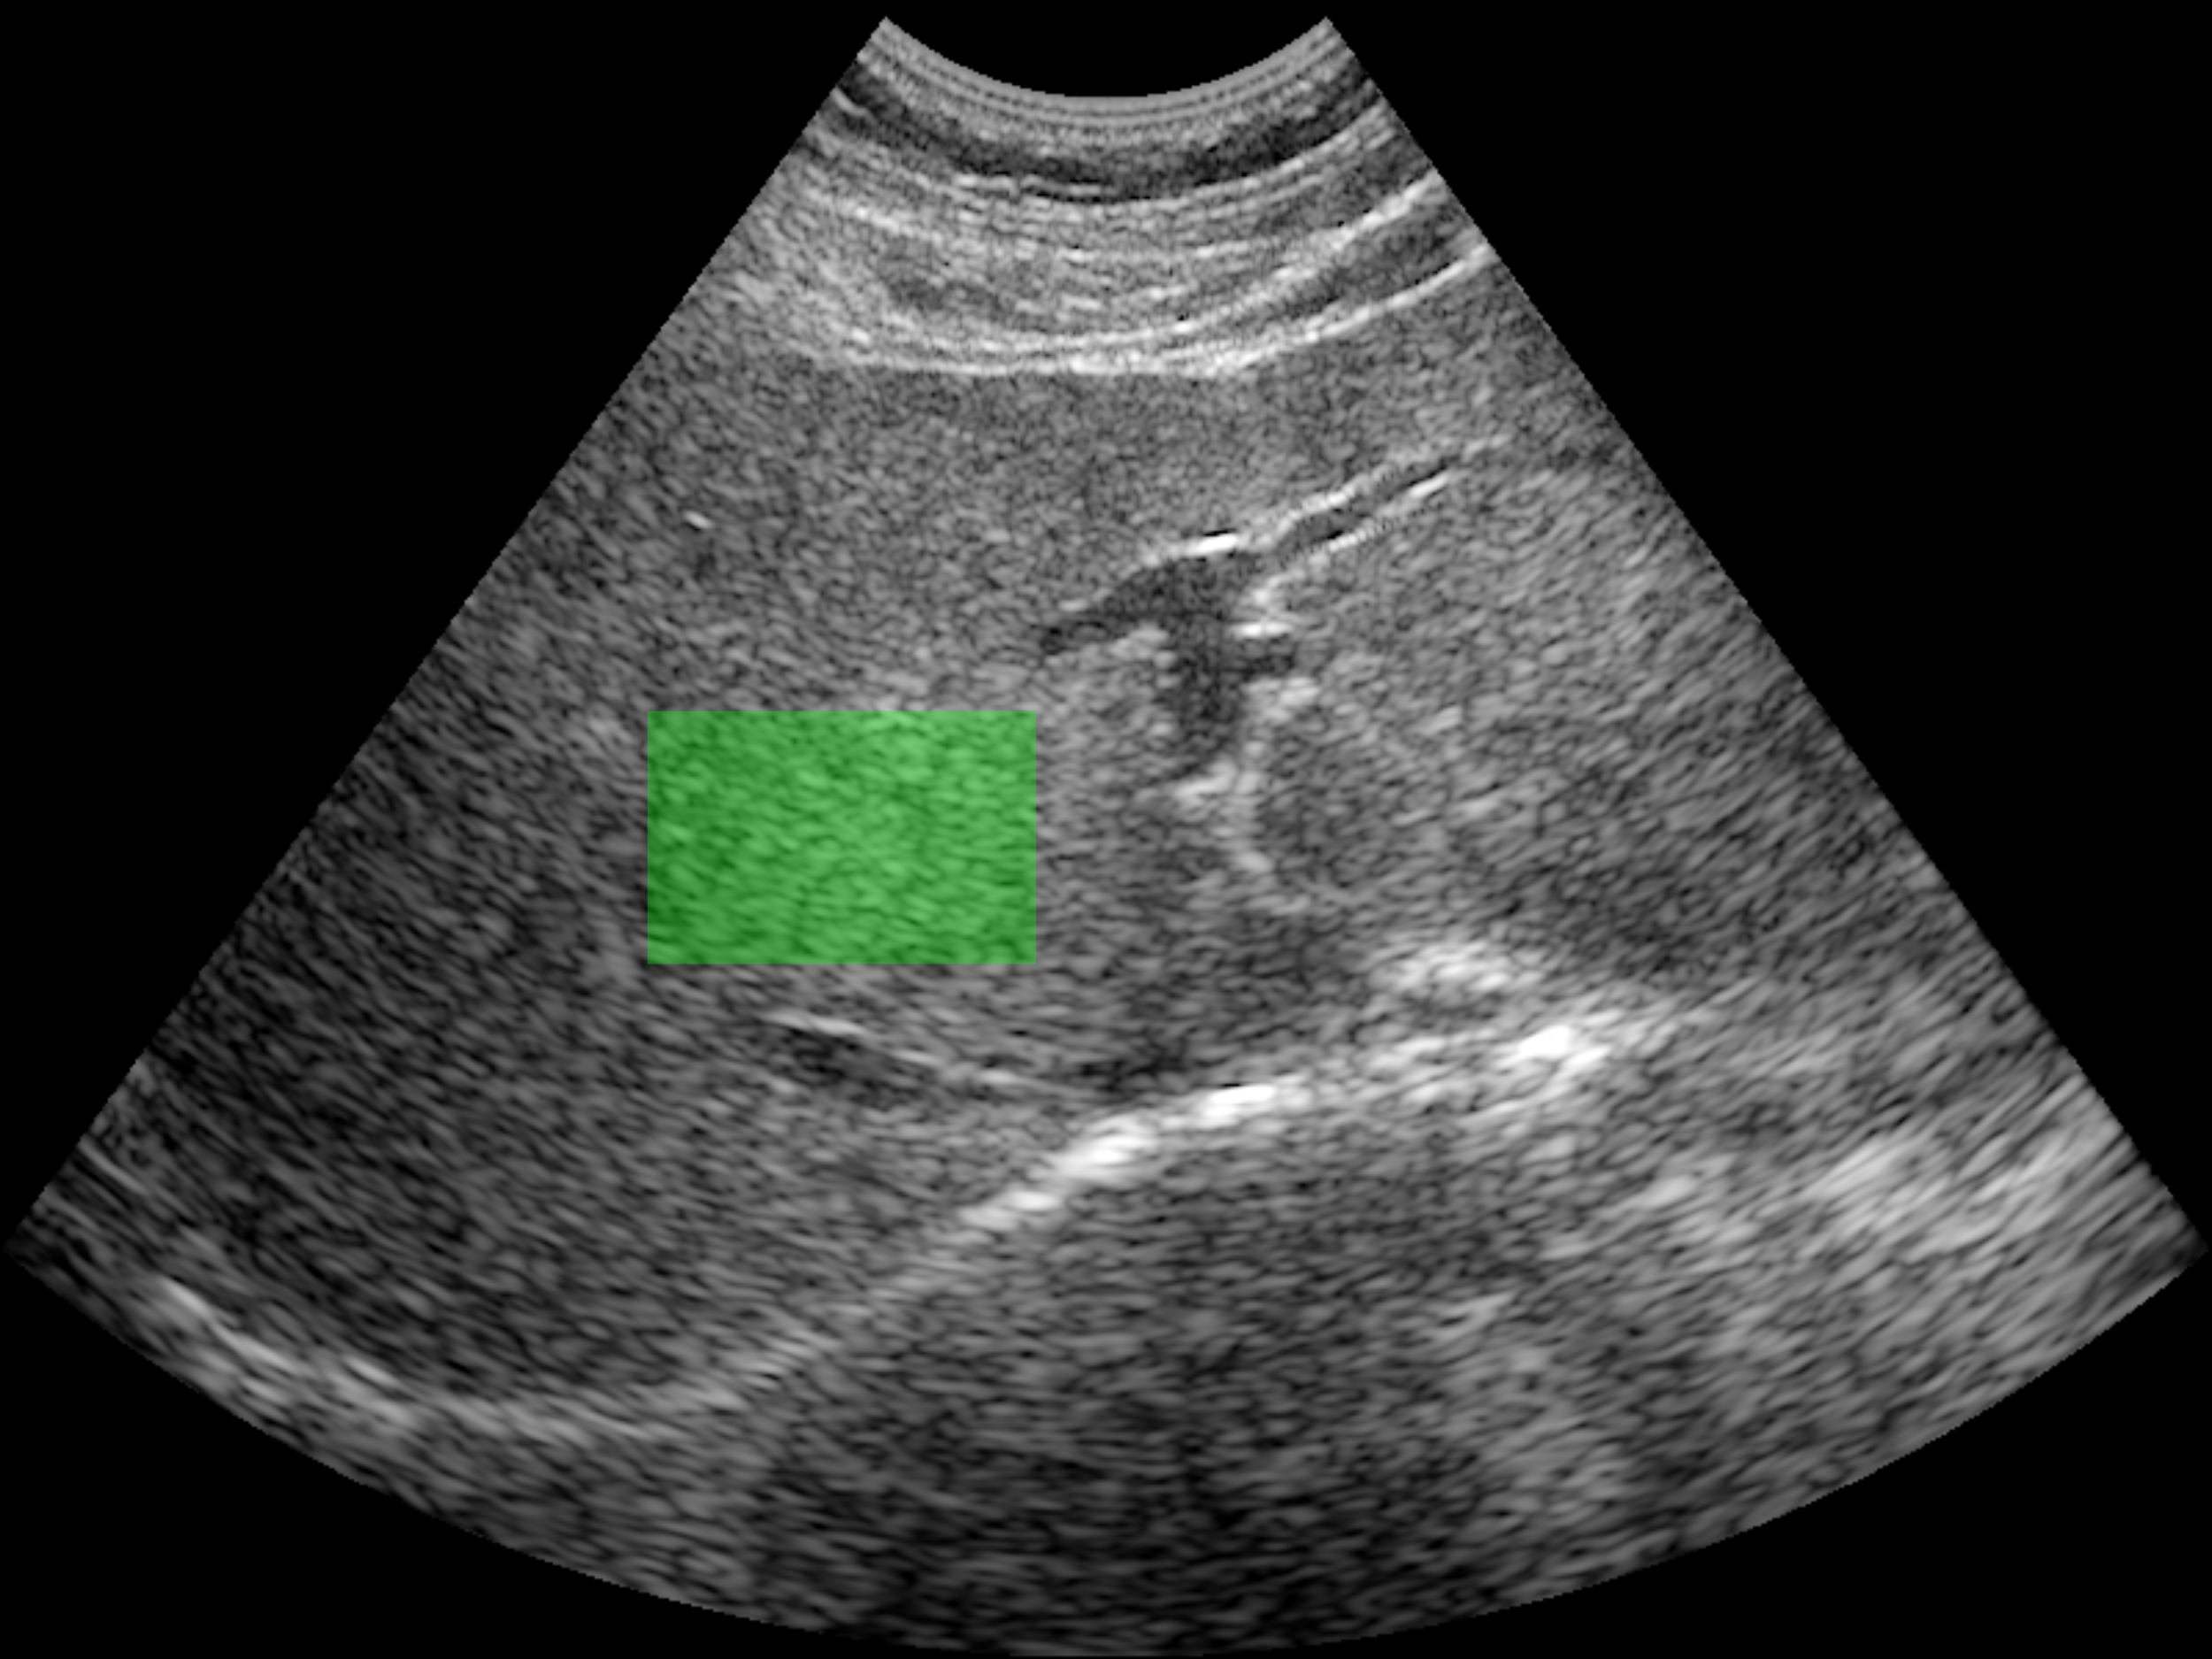
\includegraphics[height=3cm]{figures/liver_roi.png}\label{fig:liver_roi}
  }
  \subfloat[Echocardio. Apical 4-Chamber]{
    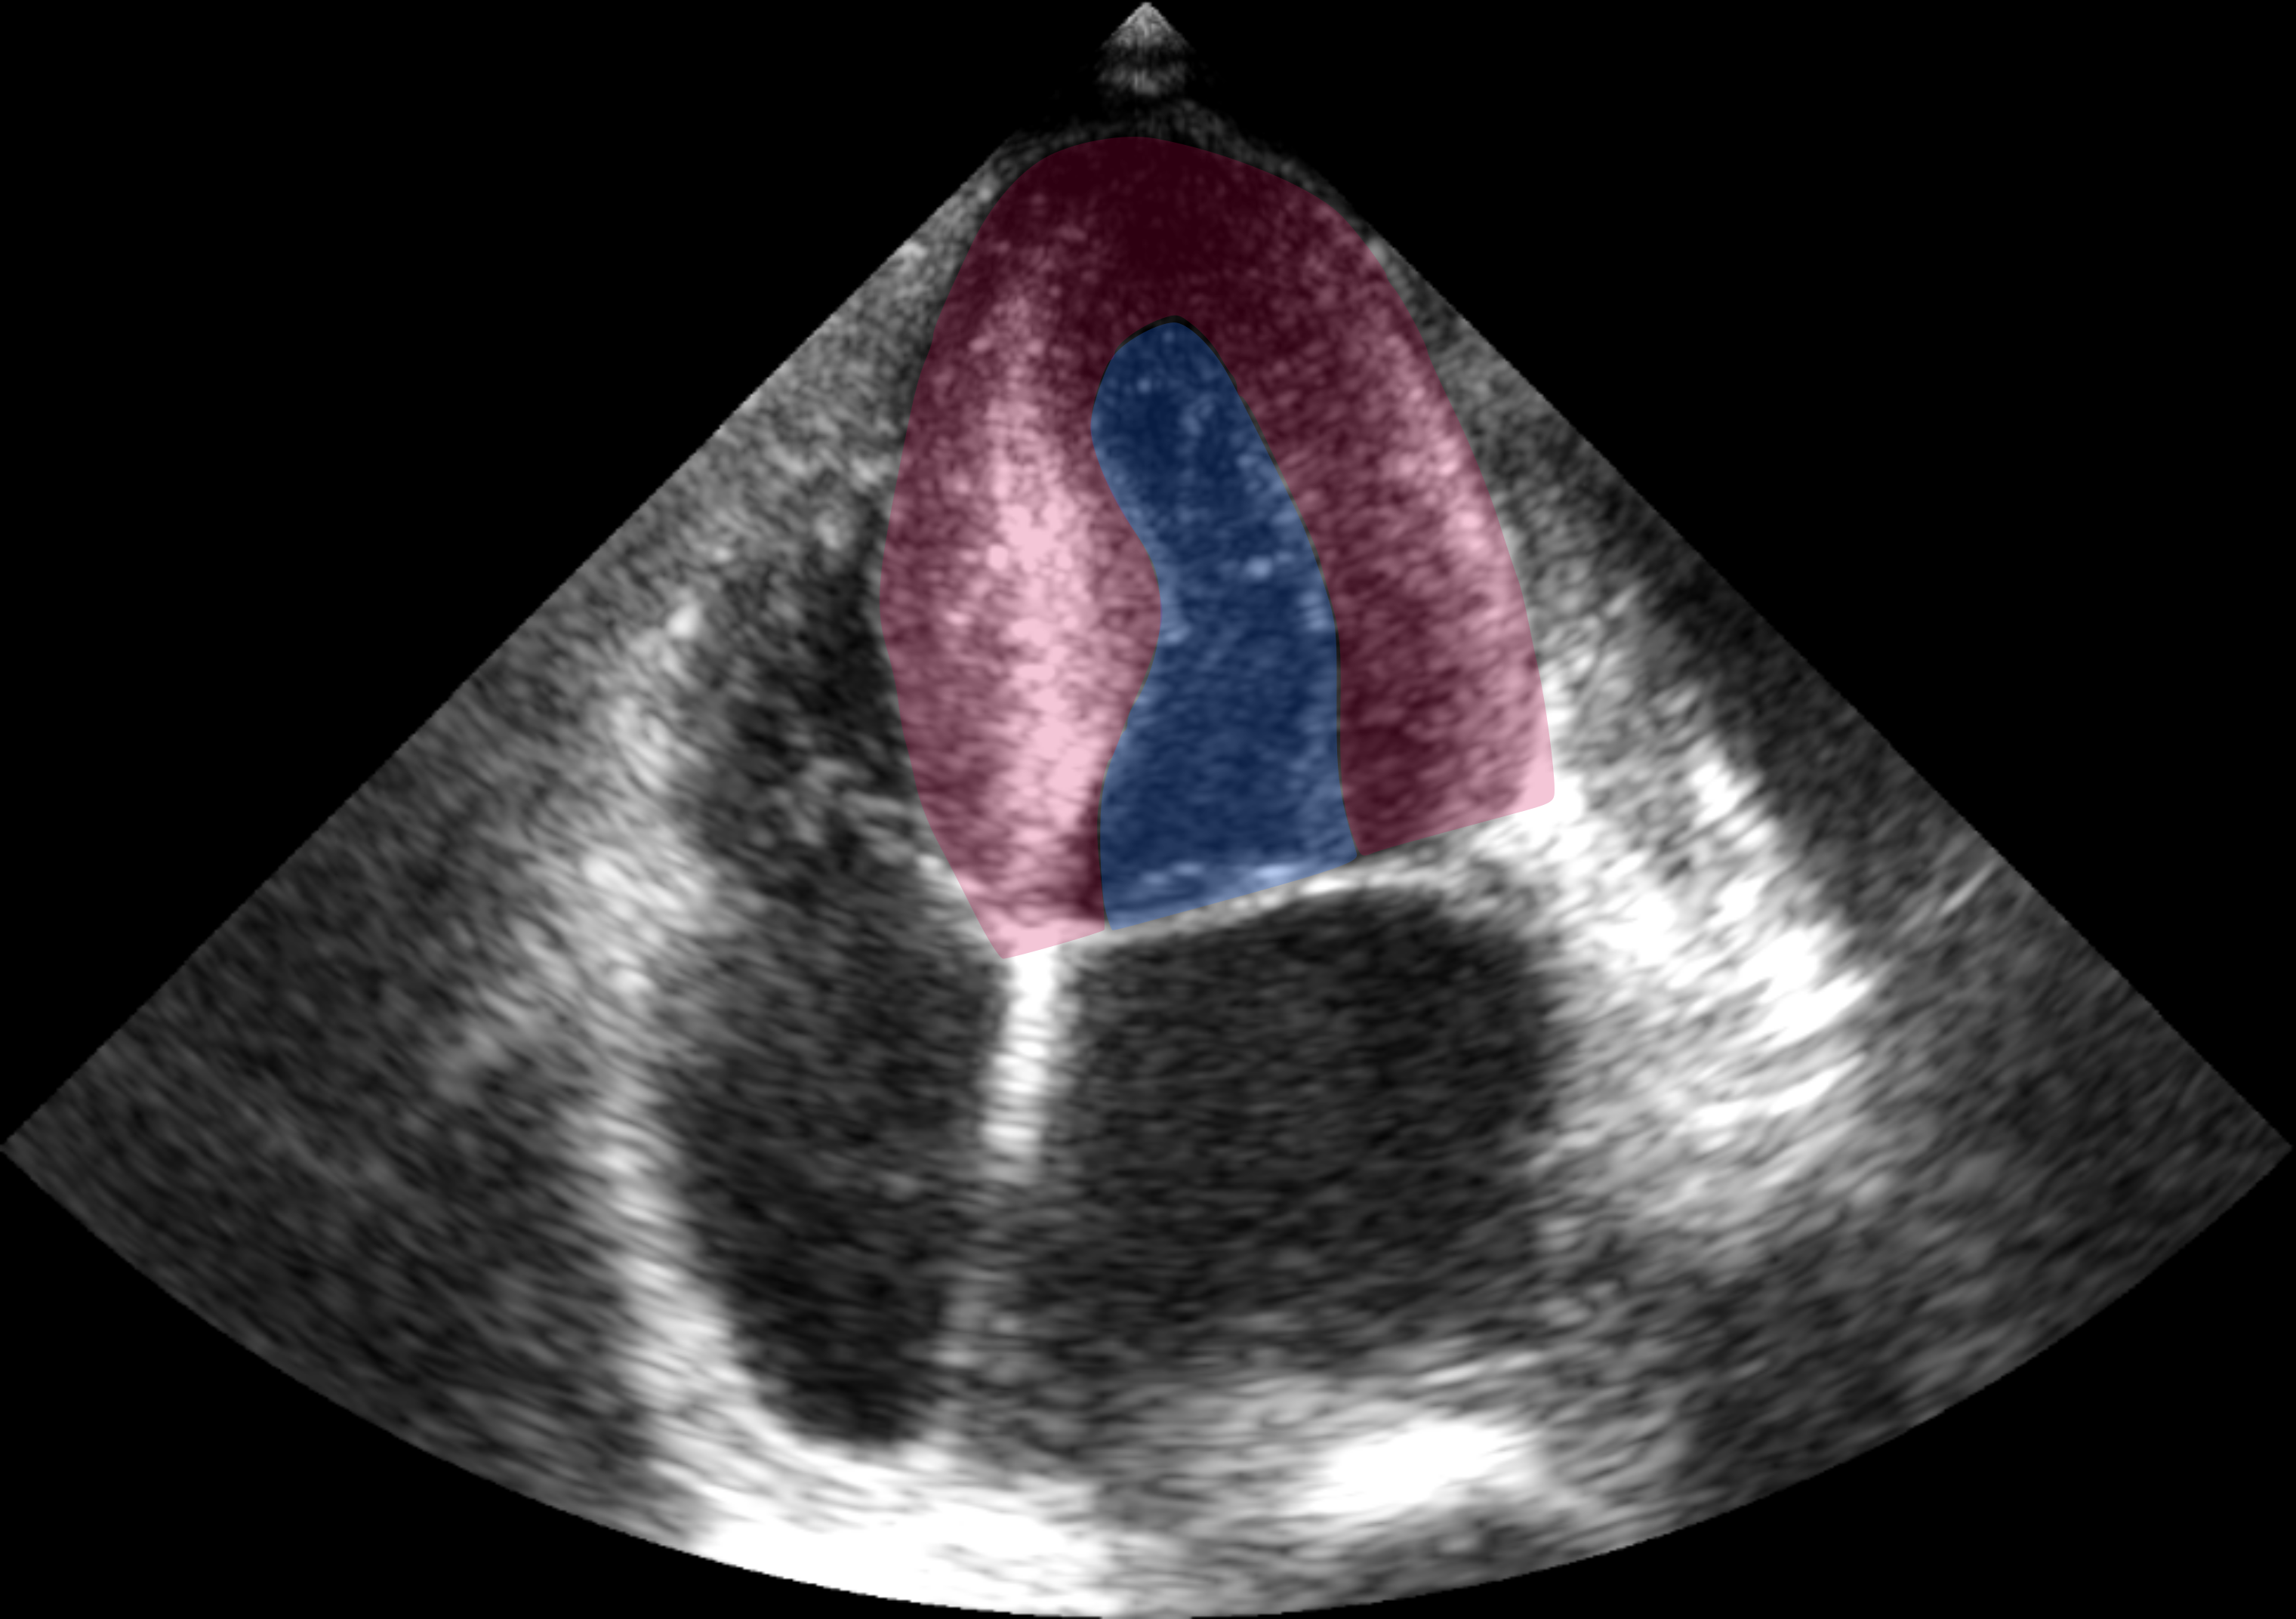
\includegraphics[height=3cm]{figures/cardiac_roi.png}\label{fig:cardiac_roi}
  }
  \caption{Regions-of-interests used for using the objective performance metrics.
    (a) The \textcolor{orange}{orange} region is used for computing the SSNR.
    (b) The \textcolor{red}{red} region (endocardium of the left ventricle) and \textcolor{blue}{blue} region (blood of the left ventricle) are used for computing the gCNR and CNR.
    The red region is also used for computing the SNR.
  }\label{fig:roi}
  \vspace{-0.1in}
\end{figure}
% 


\begin{figure*}
  \centering
  \begin{subfigure}[b]{0.15\textwidth}
    \begin{tikzpicture}[
        spy using outlines={%
          rectangle,magnification=3,size=\textwidth,
          every spy on node/.append style={transparentwindow}
        }
      ]
      \node (figA) at (0.0,0.0) {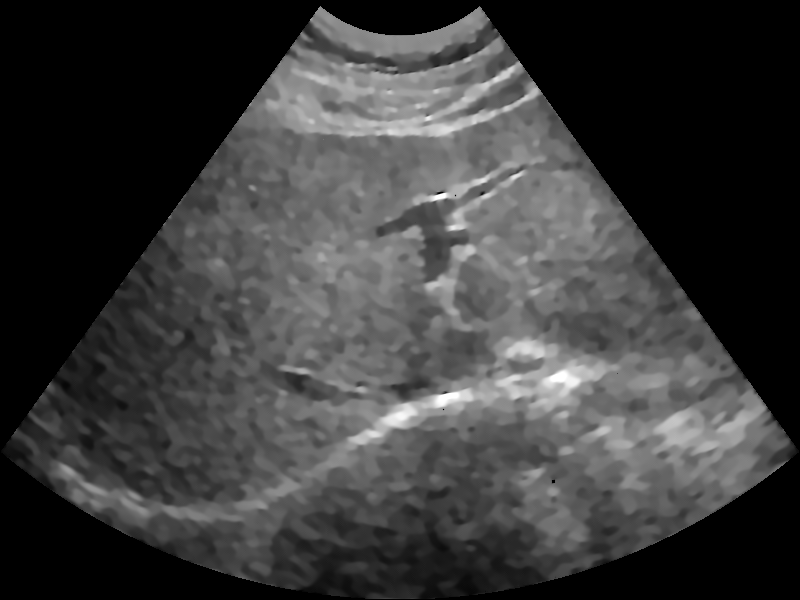
\includegraphics[width=\textwidth, trim={4cm 4cm 4cm 0cm}, clip]{figures/liver1_osrad.png}};
      \spy on (0.15, 0.0) in node [redwindow, anchor=north] at ($(figA.south)$);
    \end{tikzpicture}
    \caption{OSRAD}\label{fig:liver1_osrad}
  \end{subfigure}%
  \begin{subfigure}[b]{0.15\textwidth}
    \begin{tikzpicture}[
        spy using outlines={%
          rectangle, magnification=3,size=\textwidth,
          every spy on node/.append style={transparentwindow}
        }
      ]
      \node (figA) at (0.0,0.0) {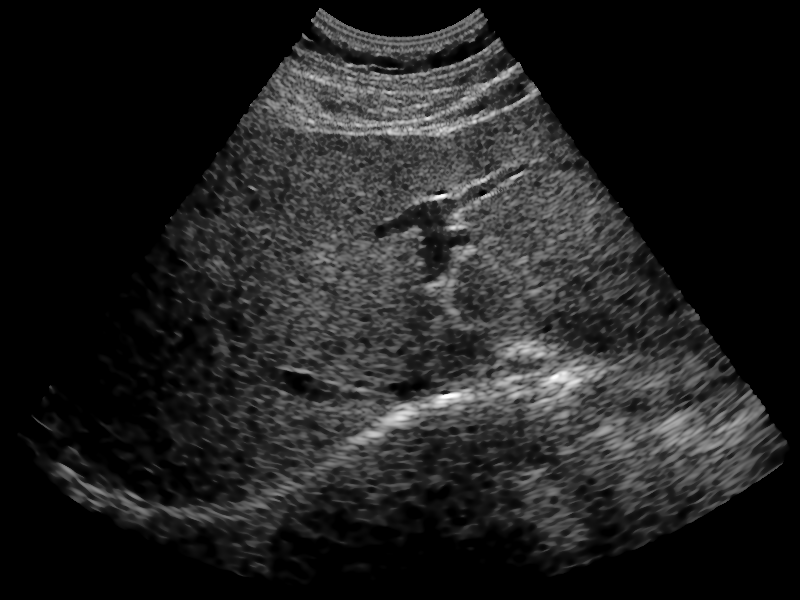
\includegraphics[width=\textwidth, trim={4cm 4cm 4cm 0cm}, clip]{figures/liver1_admss.png}};
      \spy on (0.15, 0.0) in node [redwindow, anchor=north] at ($(figA.south)$);
    \end{tikzpicture}
    \caption{ADMSS}\label{fig:liver1_admss}
  \end{subfigure}%
  \begin{subfigure}[b]{0.15\textwidth}
    \begin{tikzpicture}[
        spy using outlines={%
          rectangle, magnification=3,size=\textwidth,
          every spy on node/.append style={transparentwindow}
        }
      ]
      \node (figA) at (0.0,0.0) {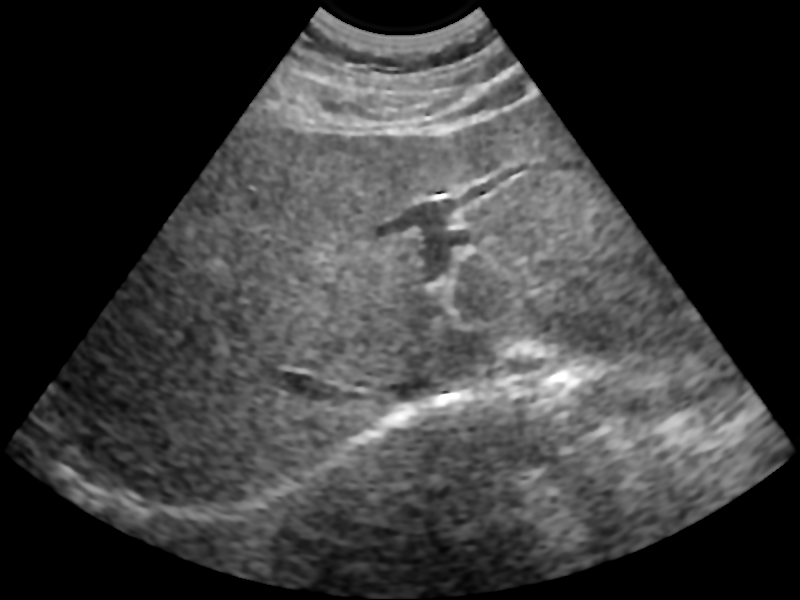
\includegraphics[width=\textwidth, trim={4cm 4cm 4cm 0cm}, clip]{figures/liver1_lpndsf.png}};
      \spy on (0.15, 0.0) in node [redwindow, anchor=north] at ($(figA.south)$);
    \end{tikzpicture}
    \caption{LPNDSF}\label{fig:liver1_lpndsf}
  \end{subfigure}%
  \begin{subfigure}[b]{0.15\textwidth}
    \begin{tikzpicture}[
        spy using outlines={%
          rectangle,magnification=3,size=\textwidth,
          every spy on node/.append style={transparentwindow}
        }
      ]
      \node (figA) at (0.0,0.0) {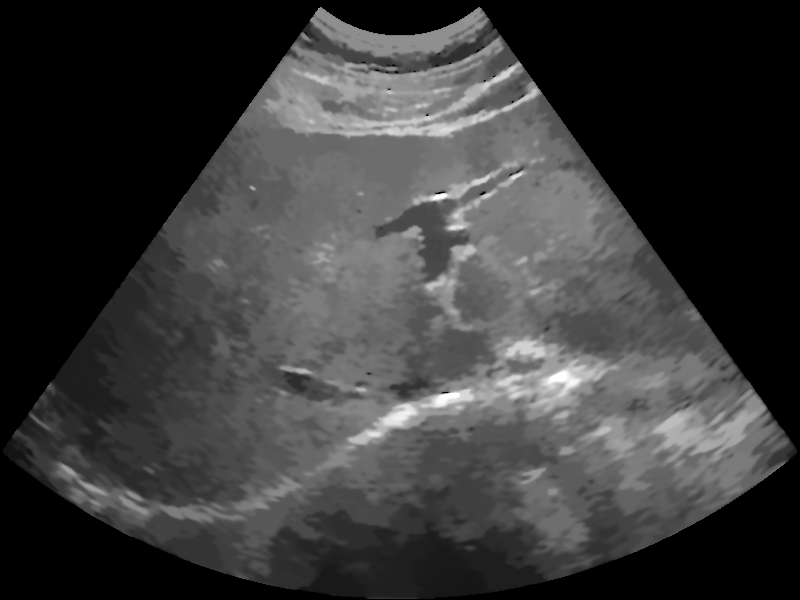
\includegraphics[width=\textwidth, trim={4cm 4cm 4cm 0cm}, clip]{figures/liver1_mnlm.png}};
      \spy on (0.15, 0.0) in node [redwindow, anchor=north] at ($(figA.south)$);
    \end{tikzpicture}
    \caption{MNLM}\label{fig:liver1_mnlm}
  \end{subfigure}%
  \begin{subfigure}[b]{0.15\textwidth}
    \begin{tikzpicture}[
        spy using outlines={%
          rectangle,magnification=3,size=\textwidth,
          every spy on node/.append style={transparentwindow}
        }
      ]
      \node (figA) at (0.0,0.0) {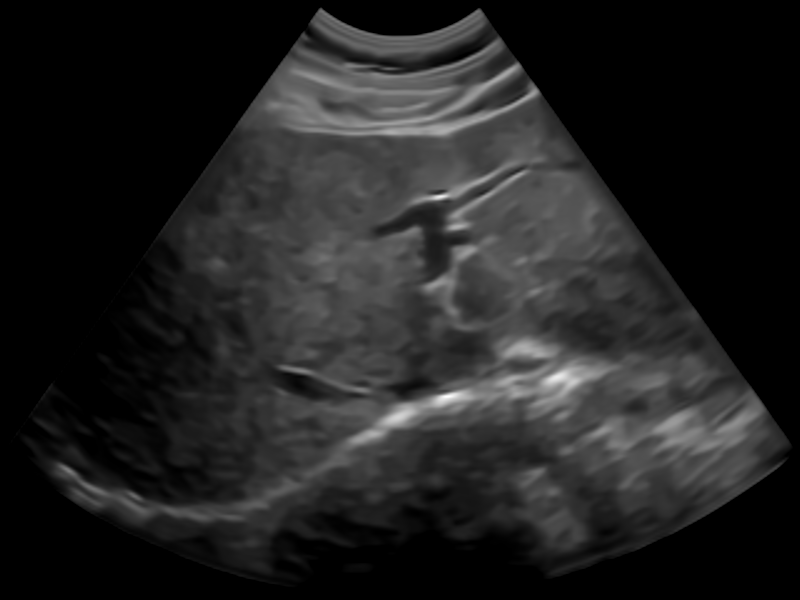
\includegraphics[width=\textwidth, trim={4cm 4cm 4cm 0cm}, clip]{figures/liver1_nllr.png}};
      \spy on (0.15, 0.0) in node [redwindow, anchor=north] at ($(figA.south)$);
    \end{tikzpicture}
    \caption{NLLR}\label{fig:liver1_nllr}
  \end{subfigure}%
  \begin{subfigure}[b]{0.15\textwidth}
    \begin{tikzpicture}[
        spy using outlines={%
          rectangle,magnification=3,size=\textwidth,
          every spy on node/.append style={transparentwindow}
        }
      ]
      \node (figA) at (0.0,0.0) {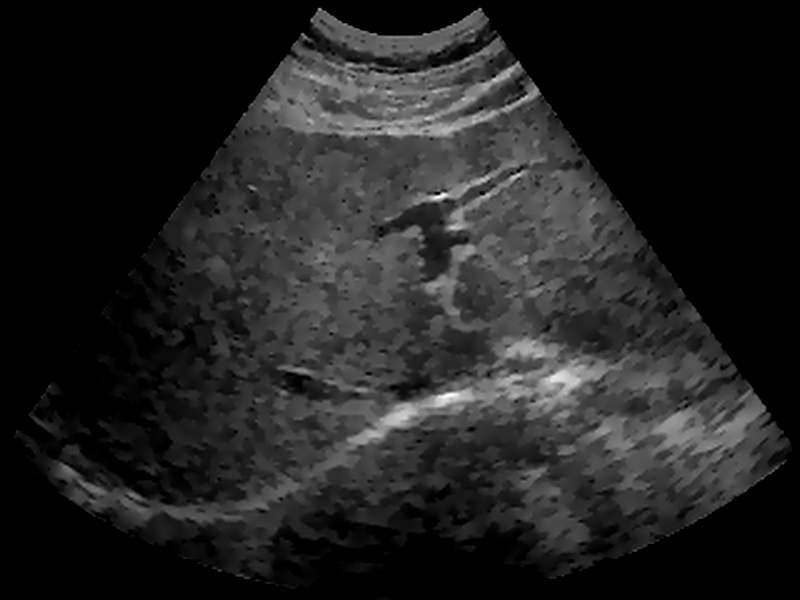
\includegraphics[width=\textwidth, trim={4cm 4cm 4cm 0cm}, clip]{figures/liver1_pfdtv.png}};
      \spy on (0.15, 0.0) in node [redwindow, anchor=north] at ($(figA.south)$);
    \end{tikzpicture}
    \caption{PFDTV}\label{fig:liver1_pfdtv}
  \end{subfigure}\\
  \begin{subfigure}[b]{0.15\textwidth}
    \begin{tikzpicture}[
        spy using outlines={%
          rectangle,magnification=3,size=\textwidth,
          every spy on node/.append style={transparentwindow}
        }
      ]
      \node (figA) at (0.0,0.0) {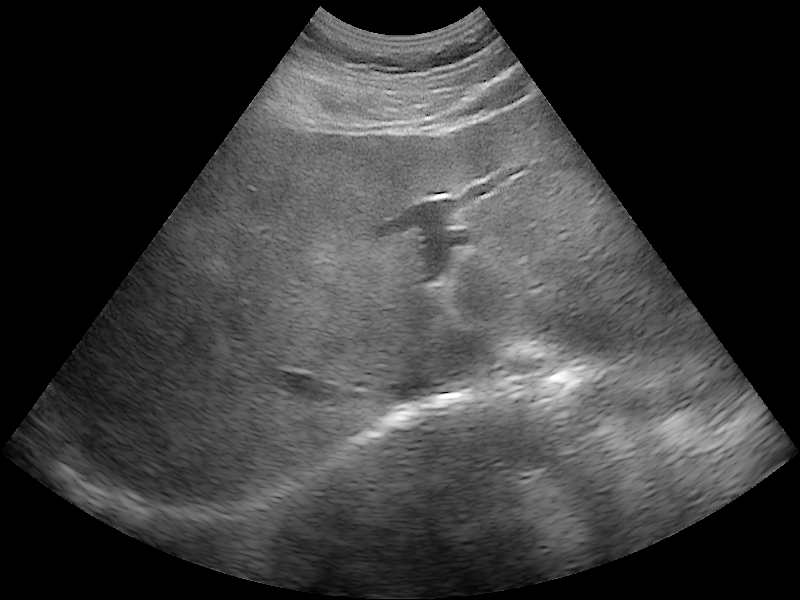
\includegraphics[width=\textwidth, trim={4cm 4cm 4cm 0cm}, clip]{figures/liver1_clpdQ.png}};
      \spy on (0.15, 0.0) in node [redwindow, anchor=north] at ($(figA.south)$);
    \end{tikzpicture}
    \caption{CLPD-SSNR}\label{fig:liver1_clpdssnr}
  \end{subfigure}%
  \begin{subfigure}[b]{0.15\textwidth}
    \begin{tikzpicture}[
        spy using outlines={%
          rectangle,magnification=3,size=\textwidth,
          every spy on node/.append style={transparentwindow}
        }
      ]
      \node (figA) at (0.0,0.0) {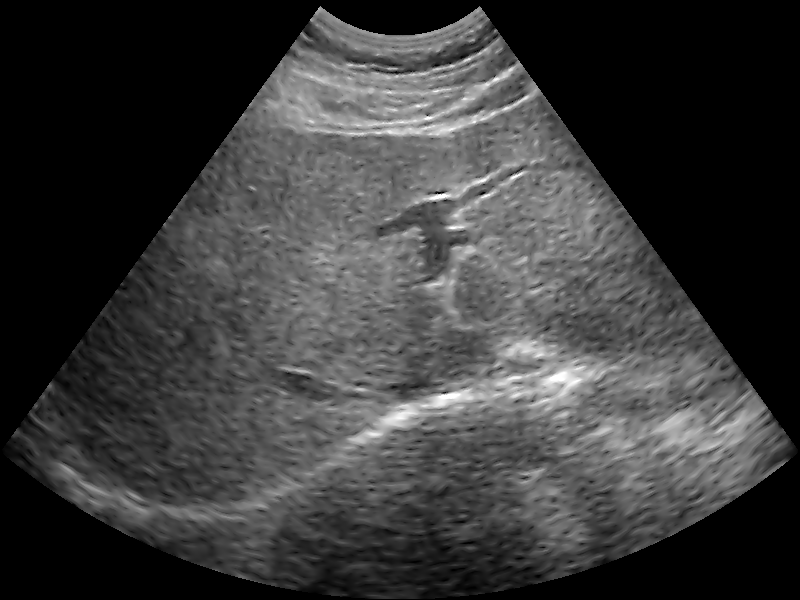
\includegraphics[width=\textwidth, trim={4cm 4cm 4cm 0cm}, clip]{figures/liver1_clpda.png}};
      \spy on (0.15, 0.0) in node [redwindow, anchor=north] at ($(figA.south)$);
    \end{tikzpicture}
    \caption{CLPD-A}\label{fig:liver1_clpda}
  \end{subfigure}%
  \begin{subfigure}[b]{0.15\textwidth}
    \begin{tikzpicture}[
        spy using outlines={%
          rectangle,magnification=3,size=\textwidth,
          every spy on node/.append style={transparentwindow}
        }
      ]
      \node (figA) at (0.0,0.0) {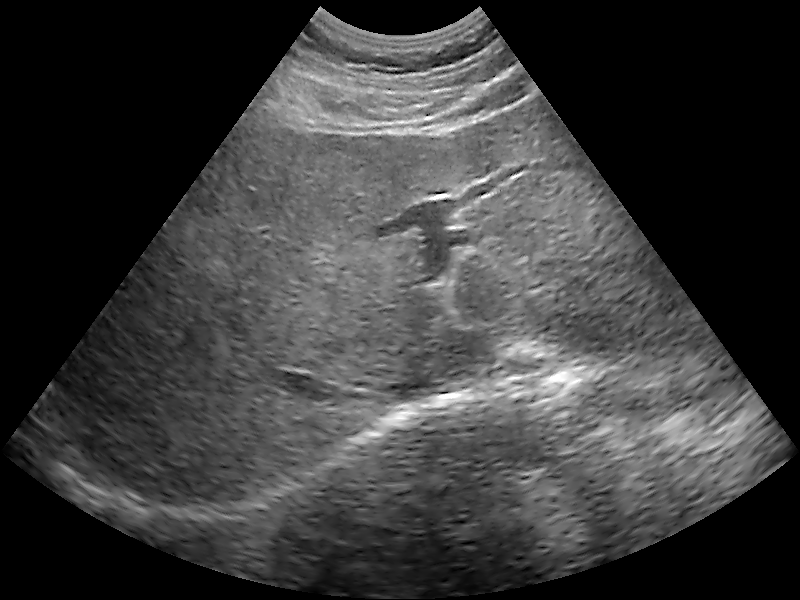
\includegraphics[width=\textwidth, trim={4cm 4cm 4cm 0cm}, clip]{figures/liver1_clpdb.png}};
      \spy on (0.15, 0.0) in node [redwindow, anchor=north] at ($(figA.south)$);
    \end{tikzpicture}
    \caption{CLPD-B}\label{fig:liver1_clpdb}
  \end{subfigure}%
  \begin{subfigure}[b]{0.15\textwidth}
    \begin{tikzpicture}[
        spy using outlines={%
          rectangle,magnification=3,size=\textwidth,
          every spy on node/.append style={transparentwindow}
        }
      ]
      \node (figA) at (0.0,0.0) {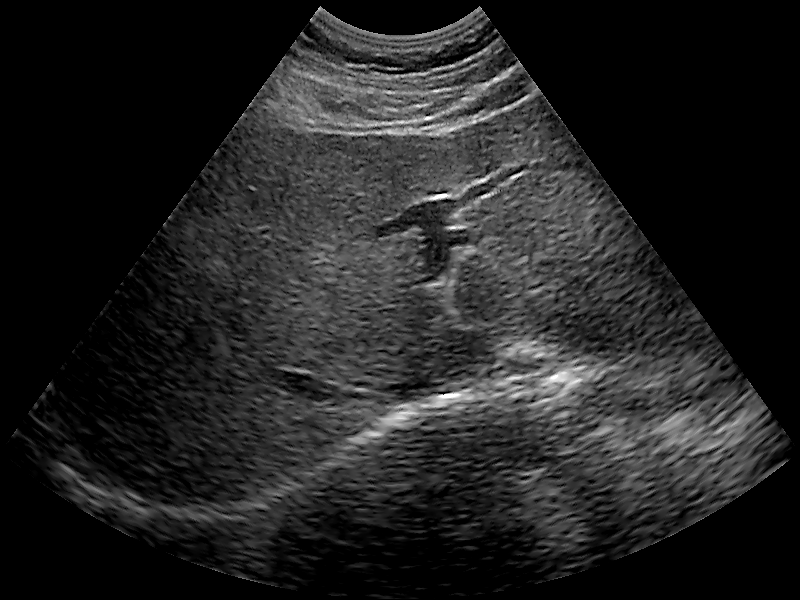
\includegraphics[width=\textwidth, trim={4cm 4cm 4cm 0cm}, clip]{figures/liver1_clpdc.png}};
      \spy on (0.15, 0.0) in node [redwindow, anchor=north] at ($(figA.south)$);
    \end{tikzpicture}
    \caption{CLPD-C}\label{fig:liver1_clpdc}
  \end{subfigure}%
  \begin{subfigure}[b]{0.15\textwidth}
    \begin{tikzpicture}[
        spy using outlines={%
          rectangle,magnification=3,size=\textwidth,
          every spy on node/.append style={transparentwindow}
        }
      ]
      \node (figA) at (0.0,0.0) {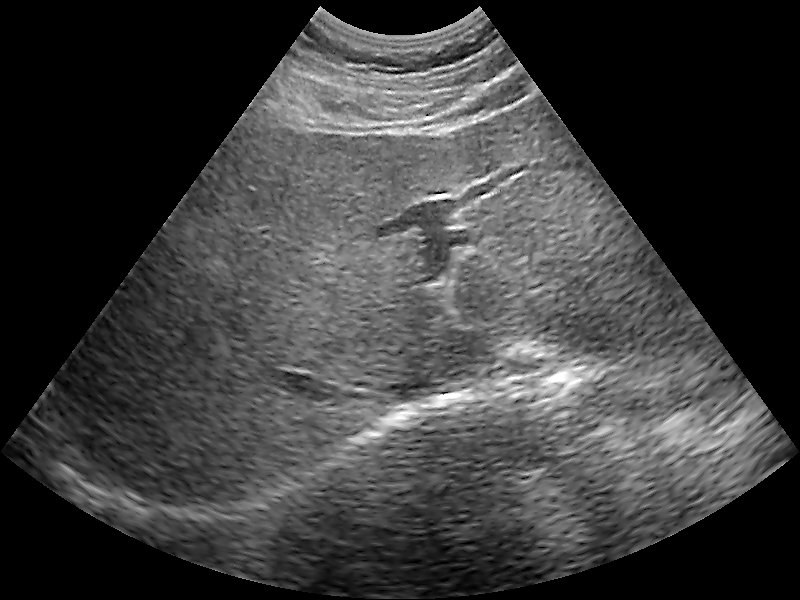
\includegraphics[width=\textwidth, trim={4cm 4cm 4cm 0cm}, clip]{figures/liver1_clpdd.png}};
      \spy on (0.15, 0.0) in node [redwindow, anchor=north] at ($(figA.south)$);
    \end{tikzpicture}
    \caption{CLPD-D}\label{fig:liver1_clpdd}
  \end{subfigure}%
  \begin{subfigure}[b]{0.15\textwidth}
    \begin{tikzpicture}[
        spy using outlines={%
          rectangle,magnification=3,size=\textwidth,
          every spy on node/.append style={redwindow}
        }
      ]
      \node (figA) at (0.0,0.0) {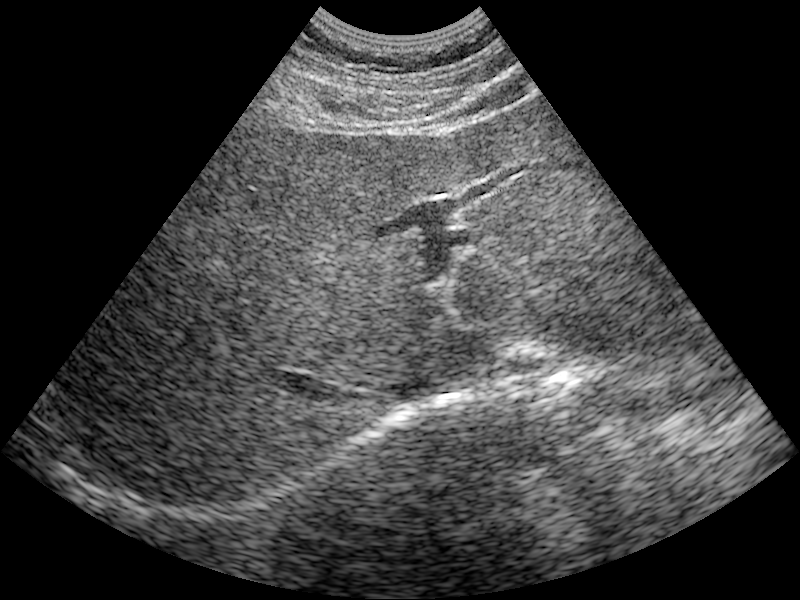
\includegraphics[width=\textwidth, trim={4cm 4cm 4cm 0cm}, clip]{figures/liver1.png}};
      \spy on (0.15, 0.0) in node [redwindow, anchor=north] at ($(figA.south)$);
    \end{tikzpicture}
    \caption{Original}\label{fig:liver_original}
  \end{subfigure}
  \caption{Results on a liver subcostal-view image.}\label{fig:liver1}
\end{figure*}

%%% Local Variables:
%%% TeX-master: "master"
%%% End:

%
\subsubsection{Metrics}
For objective quality assessment, we apply image quality metrics to the resulting images \textit{without} dynamic range adjustment.
All results are presented up to three significant digits.

\paragraph{(Speckle) Signal-to-Noise Ratio (SNR)}
The SNR measures the amount of speckle-noise relative to the mean response of a region of interest.
It is given as
\begin{align}
  \mathrm{SNR} \texttt{[dB]} = 10 \log_{10} \frac{\mu}{\sigma}
\end{align}
{\noindent}where \(\mu\) is the mean response and \(\sigma\) is the standard deviation of the region-of-interest.
When computed against a fully-formed speckle region, the SNR is called the \textit{speckle} SNR (SSNR).
In this case, \(\sigma\) corresponds to the noise standard deviation.
We present the SNR on a decibel scale.

\paragraph{Contrast-to-Noise Ratio (CNR)}
The CNR first introduced by Patterson and Foster~\cite{patterson_improvement_1983} measures the mean response difference of two regions-of-interests relative to their standard deviations, such as
\begin{align}
  \mathrm{CNR} \texttt{[dB]} = 10 \log_{10} \left(\,| \mu_{1} - \mu_{2} | \,/\, \sqrt{\sigma^2_1 + \sigma^2_2}\, \right)
\end{align}
{\noindent}where \(\mu_1, \mu_2\) are the mean responses of the regions-of-interests, and \(\sigma_1, \sigma_2\) are their standard deviations, respectively.
While the CNR is loosely related to the lesions detectibility~\cite{smith_ultrasound_1984}, Rindal \textit{et al.} has shown that it is less reliable when the dynamic range is altered~\cite{rindal_effect_2019}.
We present the CNR on a decibel scale.

%% Nonetheless, the CNR still provides a measure of relative contrast.

\paragraph{Generalized CNR (gCNR)}
As a remedy to the limitations of the CNR, Rodriguez-Molares \textit{et al.}~\cite{rodriguez-molares_generalized_2020} proposed the gCNR metric.
They showed that it is less affected by dynamic range alternations, making it a better general performance metric.
The gCNR is defined as
{
\begin{align}
  \text{gCNR} = 1 - \int_{-\infty}^{\infty} \min\big(p_1\left(x\right), p_2\left(x\right)\big) \, dx
\end{align}
}
{\noindent}where \(p_1\left(x\right)\) and \(p_2\left(x\right)\) are the probability densities of \(x\) subject to the pixel intensity distributions of the regions-of-interests 1 and 2.

\paragraph{Structural Similarity Index (SSIM)}
The SSIM is a metric for measuring the \textit{structural} similarity of images, which is derived as a product of the differences in luminance, structure, and contrast~\cite{wang_image_2004a}.
Wang \textit{et al.} have shown that the SSIM is aligned with the perception of humans and is sensitive to distortions such as blur and blockiness.
Mathematically, the SSIM between images 1 and 2 is computed such that
{
\begin{align}
  \mathrm{SSIM} = \frac{1}{N} \sum_k^N \frac{
    (2 \mu_{1,k} \, \mu_{2, k} + C_1)\,(2 \sigma_{12, k} + C_2)
  }{
    (\mu_{1,k}^2 + \mu_{2,k}^2 + C_1)\,( \sigma_{1,k}^2 + \sigma_{2,k}^2 + C_2)
  }
\end{align}
}
{\noindent}where \(\mu_{1,k}\), \(\mu_{2,k}\), are the mean of the \(k\)th patch on each images, \(\sigma_{1,k}^2\), \(\sigma_{2,k}^2\) are their respective variances, and \(\sigma_{12, k}\) is the covariance of the two.
The SSIM is taken as an average over all the patches taken by a \(11 \times 11\) Gaussian window of standard deviation 1.5.
The coefficients are chosen as \(C_1 = 1 \times 10^{-4}, C_2 = 9 \times 10^{-4} \).
We use the implementation of the \texttt{ImageQualityIndexes.jl} library\footnote{\url{https://github.com/JuliaImages/ImageQualityIndexes.jl}}


\begin{figure*}
  \vspace{-0.2in}
  \centering
  \begin{subfigure}[b]{0.15\textwidth}
    \begin{tikzpicture}[
        spy using outlines={%
          rectangle,magnification=3,size=\textwidth,
          every spy on node/.append style={transparentwindow}
        }
      ]
      \node (figA) at (0.0,0.0) {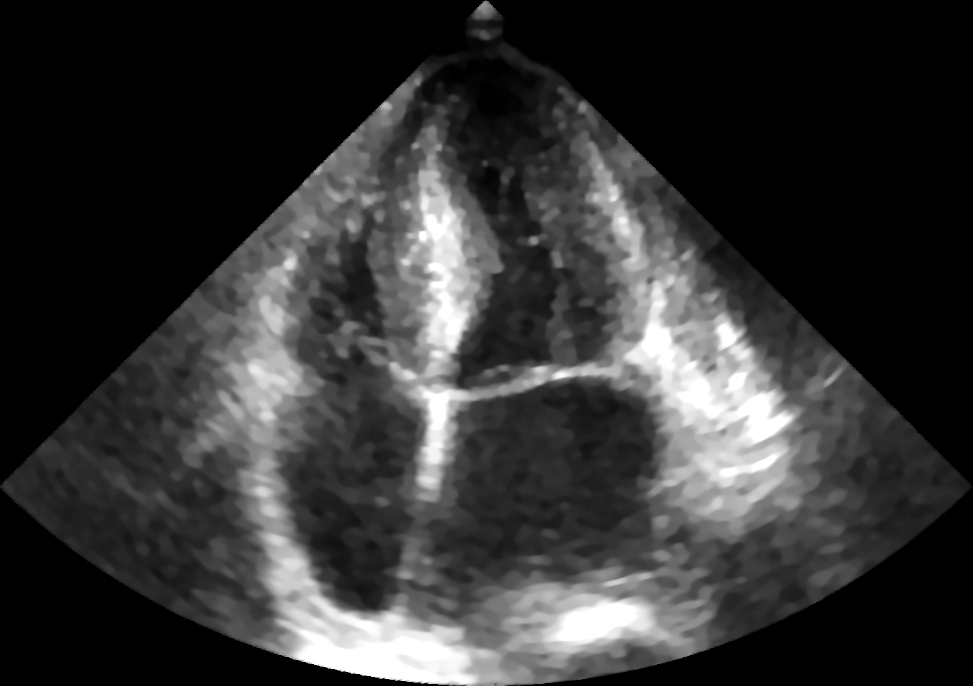
\includegraphics[width=\textwidth]{figures/cardiac3_osrad.png}};
      \spy on (0.1, 0.2) in node [redwindow, anchor=north] at ($(figA.south)$);
    \end{tikzpicture}
    \caption{OSRAD}
  \end{subfigure}%
  \begin{subfigure}[b]{0.15\textwidth}
    \begin{tikzpicture}[
        spy using outlines={%
          rectangle, magnification=3,size=\textwidth,
          every spy on node/.append style={transparentwindow}
        }
      ]
      \node (figA) at (0.0,0.0) {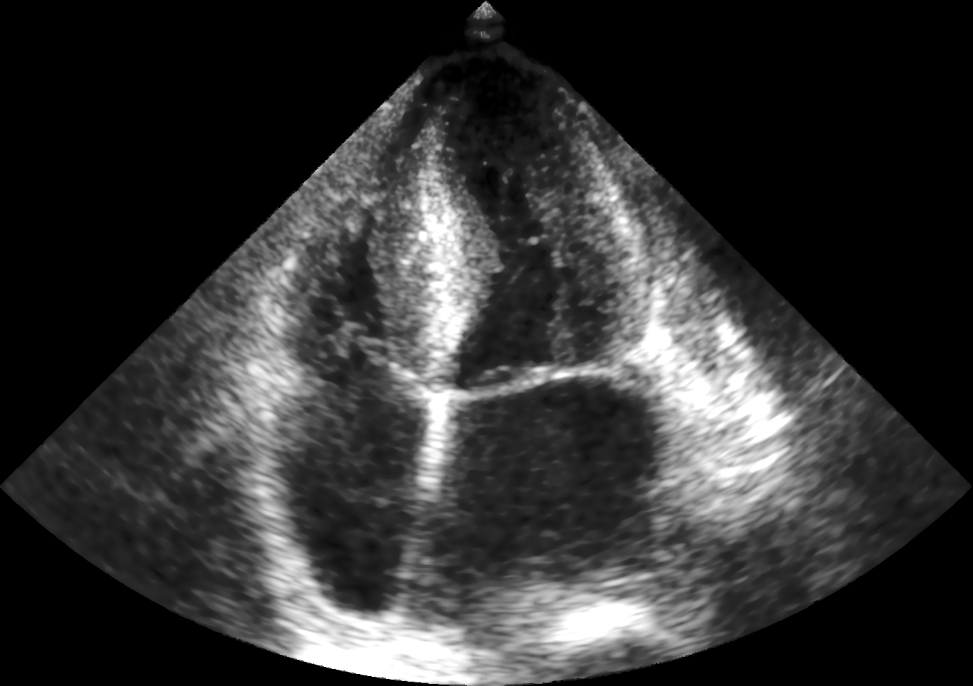
\includegraphics[width=\textwidth]{figures/cardiac3_admss.png}};
      \spy on (0.1, 0.2) in node [redwindow, anchor=north] at ($(figA.south)$);
    \end{tikzpicture}
    \caption{ADMSS}
  \end{subfigure}%
  \begin{subfigure}[b]{0.15\textwidth}
    \begin{tikzpicture}[
        spy using outlines={%
          rectangle, magnification=3,size=\textwidth,
          every spy on node/.append style={transparentwindow}
        }
      ]
      \node (figA) at (0.0,0.0) {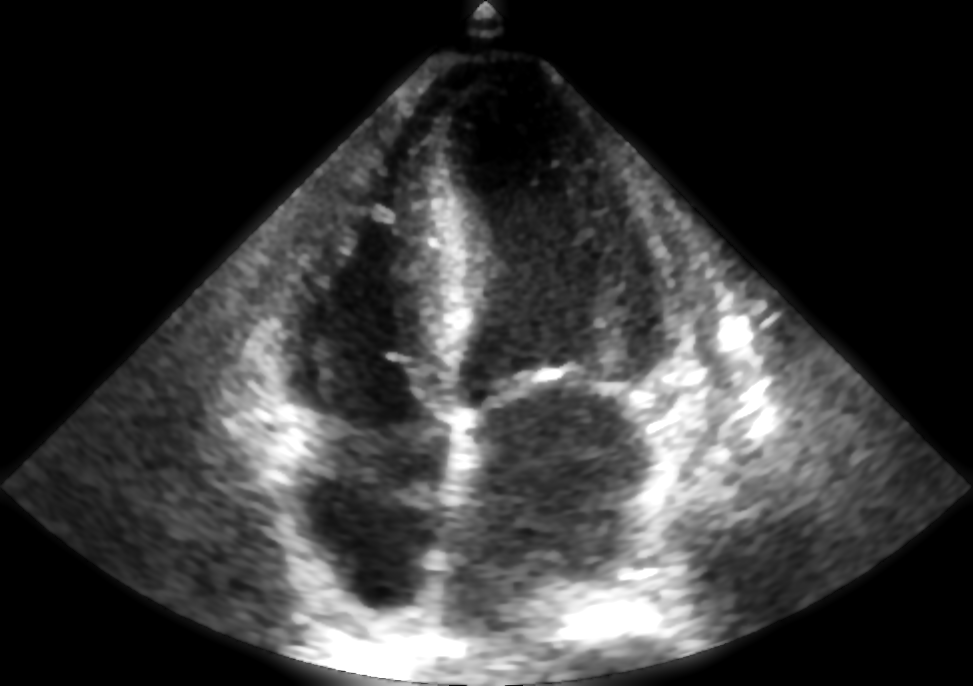
\includegraphics[width=\textwidth]{figures/cardiac3_lpndsf.png}};
      \spy on (0.1, 0.2) in node [redwindow, anchor=north] at ($(figA.south)$);
    \end{tikzpicture}
    \caption{LPNDSF}
  \end{subfigure}%
  \begin{subfigure}[b]{0.15\textwidth}
    \begin{tikzpicture}[
        spy using outlines={%
          rectangle,magnification=3,size=\textwidth,
          every spy on node/.append style={transparentwindow}
        }
      ]
      \node (figA) at (0.0,0.0) {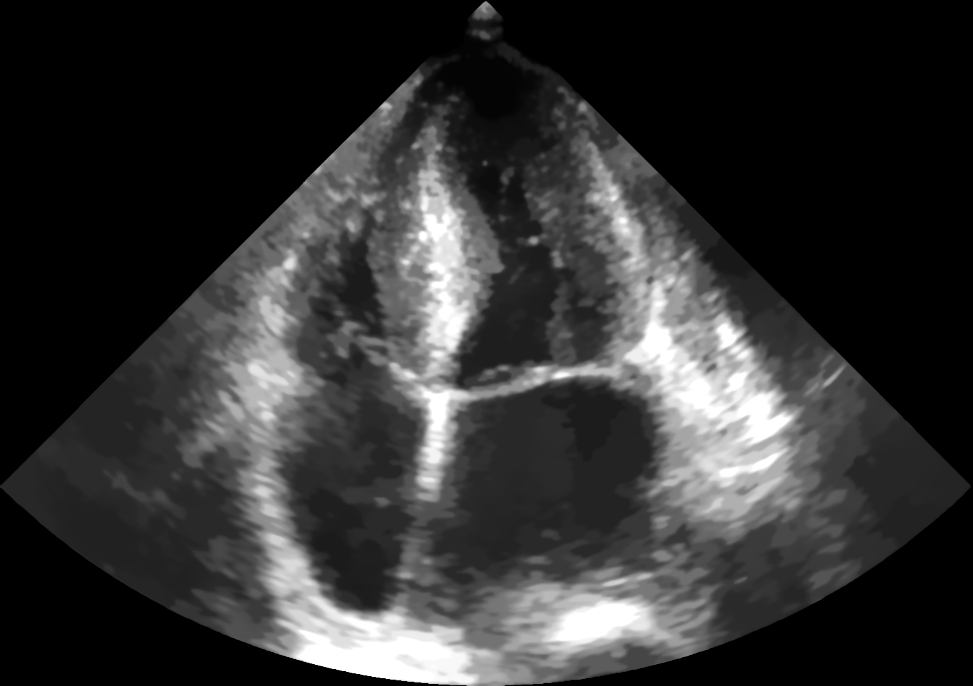
\includegraphics[width=\textwidth]{figures/cardiac3_mnlm.png}};
      \spy on (0.1, 0.2) in node [redwindow, anchor=north] at ($(figA.south)$);
    \end{tikzpicture}
    \caption{MNLM}
  \end{subfigure}%
  \begin{subfigure}[b]{0.15\textwidth}
    \begin{tikzpicture}[
        spy using outlines={%
          rectangle,magnification=3,size=\textwidth,
          every spy on node/.append style={transparentwindow}
        }
      ]
      \node (figA) at (0.0,0.0) {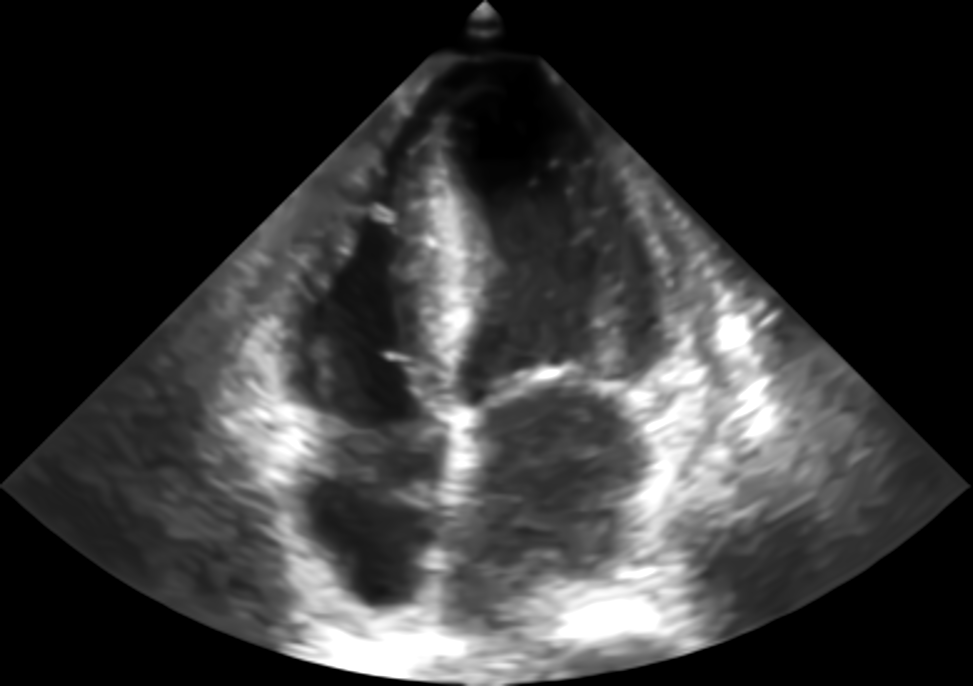
\includegraphics[width=\textwidth]{figures/cardiac3_nllr.png}};
      \spy on (0.1, 0.2) in node [redwindow, anchor=north] at ($(figA.south)$);
    \end{tikzpicture}
    \caption{NLLR}
  \end{subfigure}%
  \begin{subfigure}[b]{0.15\textwidth}
    \begin{tikzpicture}[
        spy using outlines={%
          rectangle,magnification=3,size=\textwidth,
          every spy on node/.append style={transparentwindow}
        }
      ]
      \node (figA) at (0.0,0.0) {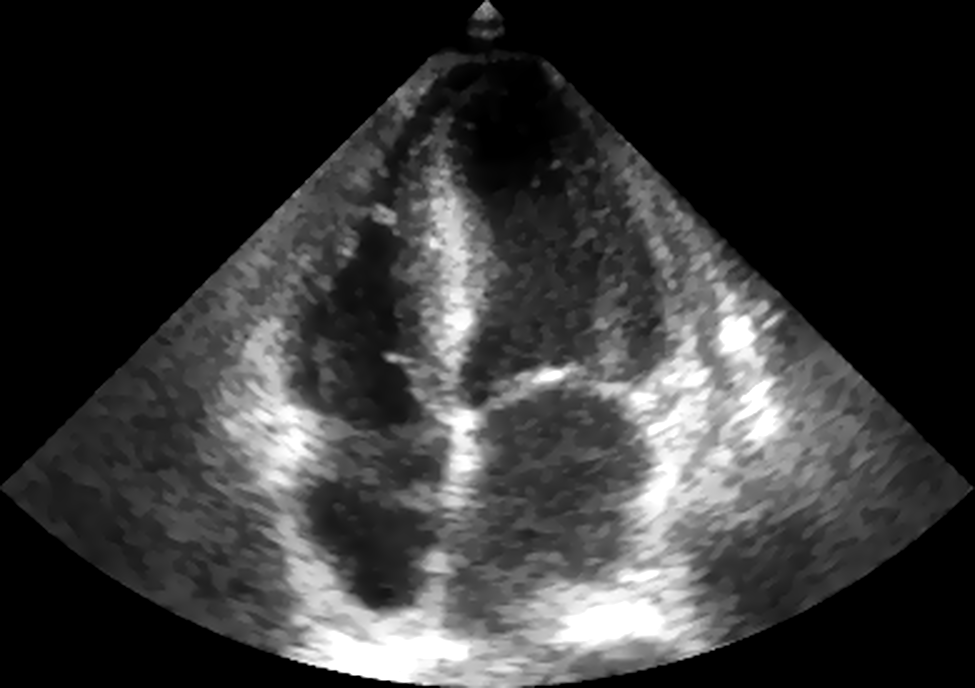
\includegraphics[width=\textwidth]{figures/cardiac3_pfdtv.png}};
      \spy on (0.1, 0.2) in node [redwindow, anchor=north] at ($(figA.south)$);
    \end{tikzpicture}
    \caption{PFDTV}
  \end{subfigure}\\
  %% \begin{subfigure}[b]{0.15\textwidth}
  %%   \begin{tikzpicture}[
  %%       spy using outlines={%
  %%         rectangle,magnification=3,size=\textwidth,
  %%         every spy on node/.append style={transparentwindow}
  %%       }
  %%     ]
  %%     \node (figA) at (0.0,0.0) {\includegraphics[width=\textwidth, trim={4cm 4cm 4cm 0cm}, clip]{figures/cardiac3_clpdQ.png}};
  %%     \spy on (0.1, 0.2) in node [redwindow, anchor=north] at ($(figA.south)$);
  %%   \end{tikzpicture}
  %%   \caption{CLPD-SSNR}
  %% \end{subfigure}%
  \begin{subfigure}[b]{0.15\textwidth}
    \begin{tikzpicture}[
        spy using outlines={%
          rectangle,magnification=3,size=\textwidth,
          every spy on node/.append style={transparentwindow}
        }
      ]
      \node (figA) at (0.0,0.0) {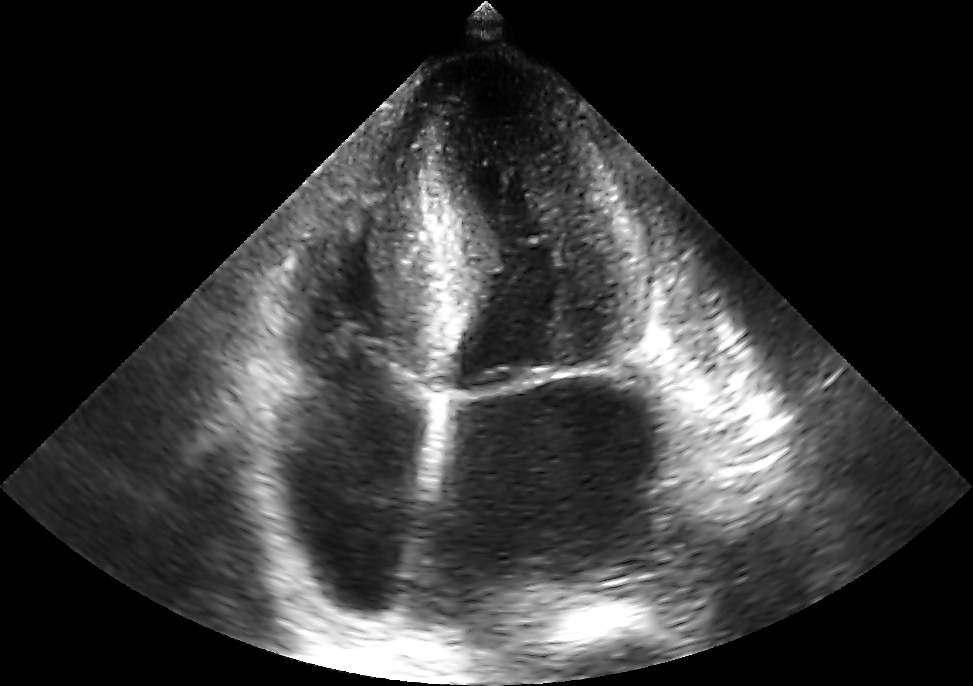
\includegraphics[width=\textwidth]{figures/cardiac3_clpda.png}};
      \spy on (0.1, 0.2) in node [redwindow, anchor=north] at ($(figA.south)$);
    \end{tikzpicture}
    \caption{CLPD-A}
  \end{subfigure}%
  \begin{subfigure}[b]{0.15\textwidth}
    \begin{tikzpicture}[
        spy using outlines={%
          rectangle,magnification=3,size=\textwidth,
          every spy on node/.append style={transparentwindow}
        }
      ]
      \node (figA) at (0.0,0.0) {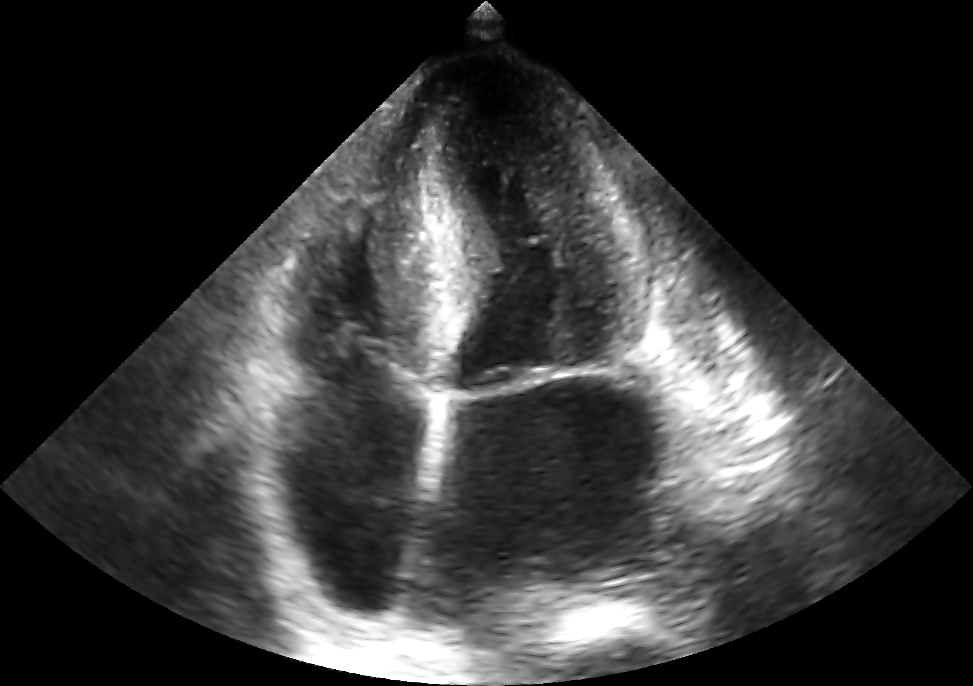
\includegraphics[width=\textwidth]{figures/cardiac3_clpdb.png}};
      \spy on (0.1, 0.2) in node [redwindow, anchor=north] at ($(figA.south)$);
    \end{tikzpicture}
    \caption{CLPD-B}
  \end{subfigure}%
  \begin{subfigure}[b]{0.15\textwidth}
    \begin{tikzpicture}[
        spy using outlines={%
          rectangle,magnification=3,size=\textwidth,
          every spy on node/.append style={transparentwindow}
        }
      ]
      \node (figA) at (0.0,0.0) {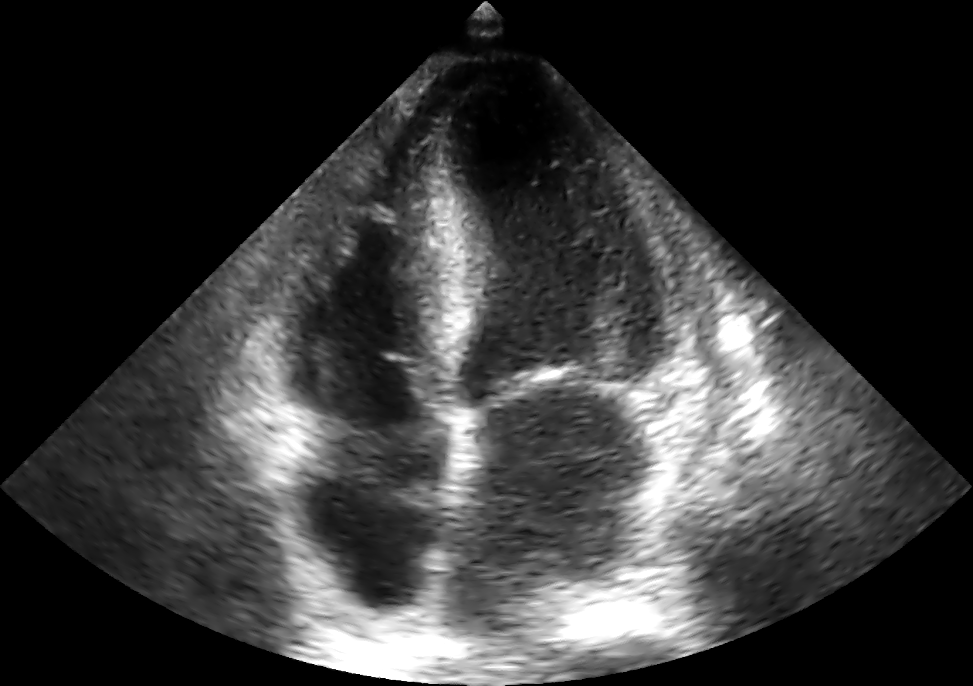
\includegraphics[width=\textwidth]{figures/cardiac3_clpde.png}};
      \spy on (0.1, 0.2) in node [redwindow, anchor=north] at ($(figA.south)$);
    \end{tikzpicture}
    \caption{CLPD-E}
  \end{subfigure}%
  \begin{subfigure}[b]{0.15\textwidth}
    \begin{tikzpicture}[
        spy using outlines={%
          rectangle,magnification=3,size=\textwidth,
          every spy on node/.append style={transparentwindow}
        }
      ]
      \node (figA) at (0.0,0.0) {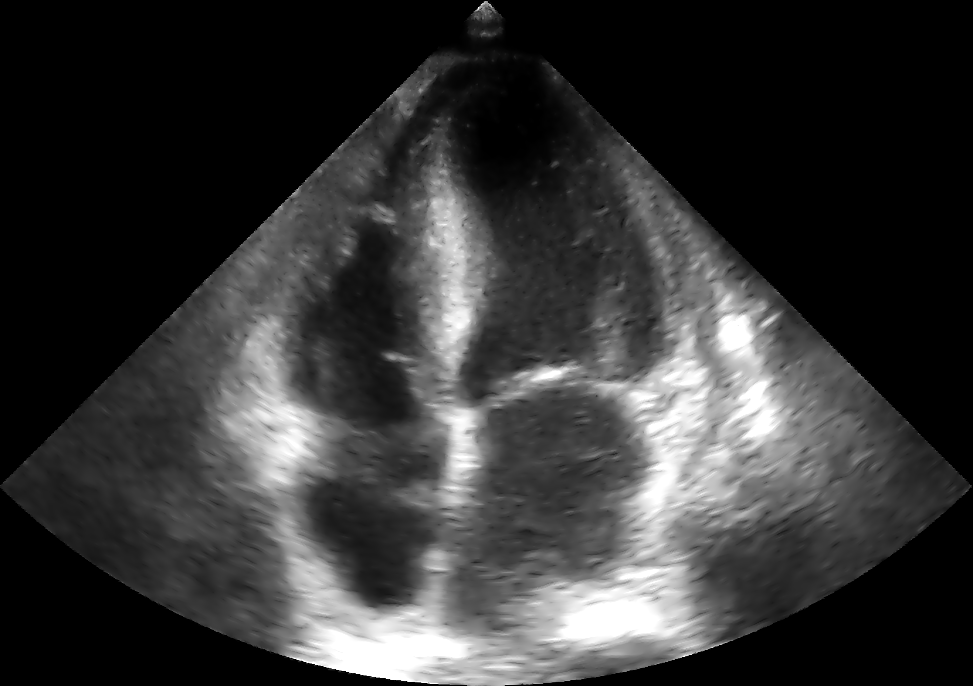
\includegraphics[width=\textwidth]{figures/cardiac3_clpdf.png}};
      \spy on (0.1, 0.2) in node [redwindow, anchor=north] at ($(figA.south)$);
    \end{tikzpicture}
    \caption{CLPD-F}
  \end{subfigure}%
  \begin{subfigure}[b]{0.15\textwidth}
    \begin{tikzpicture}[
        spy using outlines={%
          rectangle,magnification=3,size=\textwidth,
          every spy on node/.append style={redwindow}
        }
      ]
      \node (figA) at (0.0,0.0) {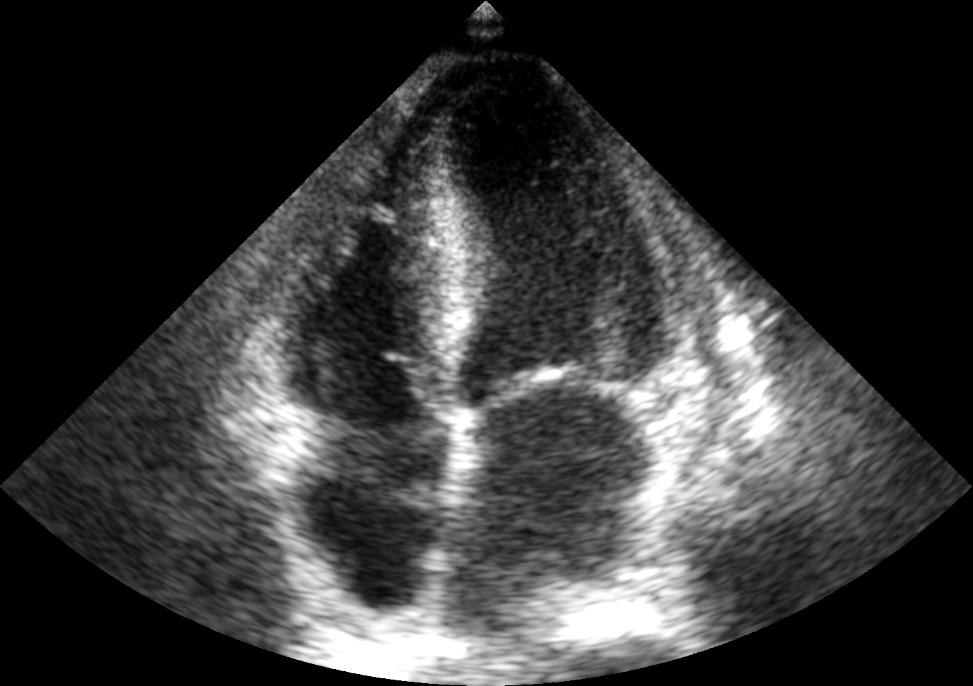
\includegraphics[width=\textwidth]{figures/cardiac3.png}};
      \spy on (0.1, 0.2) in node [redwindow, anchor=north] at ($(figA.south)$);
    \end{tikzpicture}
    \caption{Original}\label{fig:cardiac3_original}
  \end{subfigure}
  \caption{
    Results on echocardiographic 4-chamber view.
    The red squares are zooming on the left-ventricle.
  }\label{fig:cardiac3}
  \vspace{-0.15in}
\end{figure*}

%
\paragraph{\(S_3\) Index}
Finally, we use a metric for evaluating the blurriness of the images.
Blurriness metrics have not been traditionally used for evaluating the quality of medical ultrasound images.
But, we will later show that blurriness is a critical quality factor for sonographers.
In this work, we use the \(S_3\) metric proposed in~\cite{vu_bf_2012}.
The \(S_3\) value of the \(k\)th patch is defined as a harmonic mean such that
\begin{align}
  S_3\left(k\right) = \sqrt{S_1\left(k\right)} \sqrt{S_2\left(k\right)}
\end{align}
{\noindent}where \(S_1\left(k\right)\) and \(S_2\left(k\right)\) are its spatial and spectral measures of sharpness.
The final \(S_3\) index of an image is given as the average of the top 1\% \(S_3\) values.
We use the official implementation\footnote{\url{https://sites.google.com/site/cuongvt101/research/Sharpness-measure}}.

%\paragraph{Regions-of-Interests}
The regions-of-interests used for computing the performance metrics are shown in~\cref{fig:roi}.
For the liver subcostal view, we compute the metrics over multiple frames, while for the echocardiographic apical 4-chamber view, we compute them only on one representative frame.

\begin{table}
  \centering
  \caption{Quantitative Results on a Liver Subcostal View}\label{table:liver1}
  \begin{threeparttable}
  \setlength{\tabcolsep}{3.5pt}
  \begin{tabular}{llrrr}
    \toprule
    & \multicolumn{1}{c}{\textbf{Algorithm}}
    & \multicolumn{1}{c}{\textbf{SSNR} \texttt{[dB]}}
    & \multicolumn{1}{c}{\textbf{SSIM}}
    & \multicolumn{1}{c}{\(\mathbf{S_{3}}\)} \\\midrule
    \multirow{6}{*}{\footnotesize{Baselines}} & OSRAD & \textbf{20.8 {\tiny(20.3, 21.2)}} & 0.792 {\tiny(0.791, 0.794)} & 0.476 {\tiny(0.473, 0.481)}\\
    & ADMSS & 16.9 {\tiny(16.5, 17.4)} & \textbf{0.927 {\tiny(0.893, 0.963)}} & 0.350 {\tiny(0.347, 0.353)} \\
    & LPNDSF & 19.7 {\tiny(19.4, 20.0)} & 0.763 {\tiny(0.762, 0.764)}         & 0.343 {\tiny(0.340, 0.346)} \\
    & MNLM & \textbf{22.1 {\tiny(21.6, 22.7)}} & 0.811 {\tiny(0.809, 0.812)}  & 0.033 {\tiny(0.329, 0.342)} \\
    & NLLR & \textbf{22.0 {\tiny(21.6, 22.5)}} & 0.764 {\tiny(0.762, 0.765)}  & 0.141 {\tiny(0.140, 0.142)} \\
    & PFDTV & \textbf{20.0 {\tiny(19.6, 20.4)}} & 0.822 {\tiny(0.820, 0.823)} & 0.461 {\tiny(0.456, 0.465)} \\
\cdashlinelr{1-5}
    \multirow{5}{*}{\footnotesize{This work}} & CLPD-{\scriptsize{SSNR}}  & \textbf{21.0 {\tiny(20.7, 21.4)}} & \textbf{0.914 {\tiny(0.913, 0.914)}} & \textbf{0.509 {\tiny(0.507, 0.511)}} \\
    & CLPD-A  & 19.9 {\tiny(19.6, 20.2)} & 0.883 {\tiny(0.882, 0.884)} & \textbf{0.490 {\tiny(0.486, 0.494)}} \\
    & CLPD-B  & 19.8 {\tiny(19.6, 20.2)} & \textbf{0.913 {\tiny(0.913, 0.914)}} & \textbf{0.507 {\tiny(0.503, 0.511)}} \\
    & CLPD-C  & 18.2 {\tiny(18.0, 18.5)} & \textbf{0.954 {\tiny(0.953, 0.954)}} & \textbf{0.587 {\tiny(0.581, 0.592)}} \\
    & CLPD-D & 19.0 {\tiny(18.7, 19.3)} & \textbf{0.933 {\tiny(0.932, 0.933)}} &  \textbf{0.565 {\tiny(0.562, 0.569)}} \\\bottomrule
  \end{tabular}
  \begin{tablenotes}
    \item[*] We report the average, 10\%, and \%90 percentiles of the metrics taken over 16 frames.
    \item[*] The performance of the top 5 algorithms for each metric is shown in boldface.
  \end{tablenotes}
  \end{threeparttable}
  \vspace{-0.1in}
\end{table}
%
\subsection{Results on Liver Subcostal View}
%We first present experimental results with a liver subcostal view image sequence.
For the liver subcostal view experiment, we include CLPD-SSNR which was mechanically tuned to maximize both the SSNR and SSIM metric using vanilla BO.

\subsubsection{Qualitative Results}
A representative frame processed by each method is shown in~\cref{fig:liver1}.
The CLPDs tuned by sonographers (CLPD-A to CLPD-D) do not exhibit much speckle reduction.
Notice the contrast with CLPD-SSNR, which has been tuned to obtain the least speckle.
This shows that sonographers find speckle reduction less relevant to the clinical quality of liver images.
Among the CLDPs tuned by sonographers, CLPD-B shows the least speckle, reflecting the preferential difference among sonographers.
On the other hand, MNLM and NLLR showed the least speckle, but NLLR resulted in blurry images.

When focusing on blurriness and sharpness, the expert tuned CLPDs show the best results.
The edges of the left portal vein are noticeably sharper on CLPD-C and CLPD-D.
In contrast, most of the considered baselines except for ADMSS and MNLM are notably blurry.
Meanwhile, OSRAD, LPNDSF, and PFDTV results in ``blocky'' patterns, possibly because of the strong presence of pepper noise. 
Especially, ADMSS showed \textit{increased} speckle due to peppers.
The probabilistic model of ADMSS misspecified peppers as background, resulting in their exaggeration.


\begin{figure*}
  \vspace{-0.1in}
  \centering
  \begin{subfigure}[b]{0.15\textwidth}
    \begin{tikzpicture}[
        spy using outlines={%
          rectangle,magnification=3,size=\textwidth,
          every spy on node/.append style={transparentwindow}
        }
      ]
      \node (figA) at (0.0,0.0) {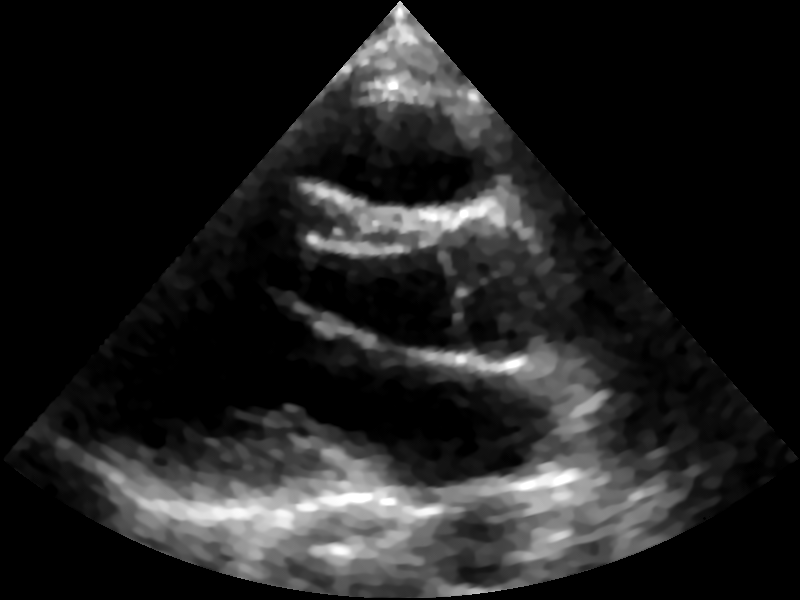
\includegraphics[width=\textwidth]{figures/cardiac1_osrad.png}};
      \spy on (0.05, 0.05) in node [redwindow, anchor=north] at ($(figA.south)$);
    \end{tikzpicture}
    \caption{OSRAD}
  \end{subfigure}%
  \begin{subfigure}[b]{0.15\textwidth}
    \begin{tikzpicture}[
        spy using outlines={%
          rectangle, magnification=3,size=\textwidth,
          every spy on node/.append style={transparentwindow}
        }
      ]
      \node (figA) at (0.0,0.0) {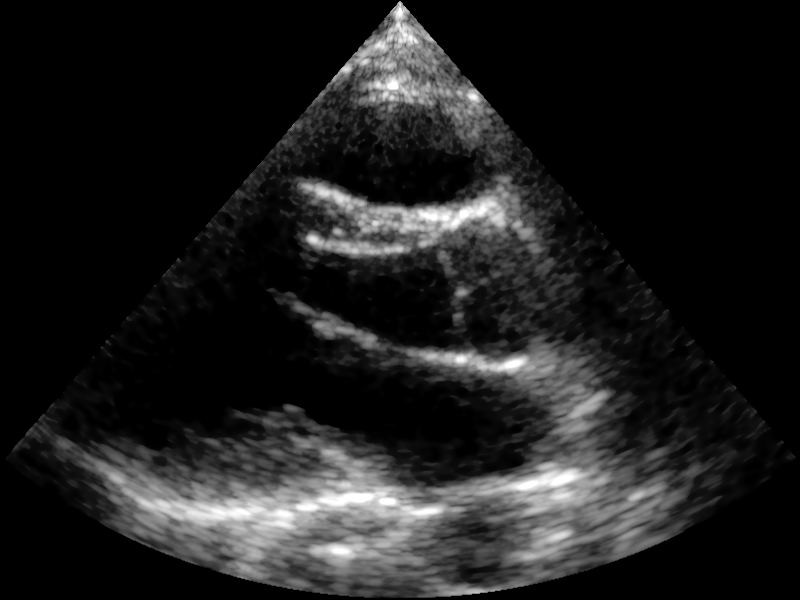
\includegraphics[width=\textwidth]{figures/cardiac1_admss.png}};
      \spy on (0.05, 0.05) in node [redwindow, anchor=north] at ($(figA.south)$);
    \end{tikzpicture}
    \caption{ADMSS}
  \end{subfigure}%
  \begin{subfigure}[b]{0.15\textwidth}
    \begin{tikzpicture}[
        spy using outlines={%
          rectangle, magnification=3,size=\textwidth,
          every spy on node/.append style={transparentwindow}
        }
      ]
      \node (figA) at (0.0,0.0) {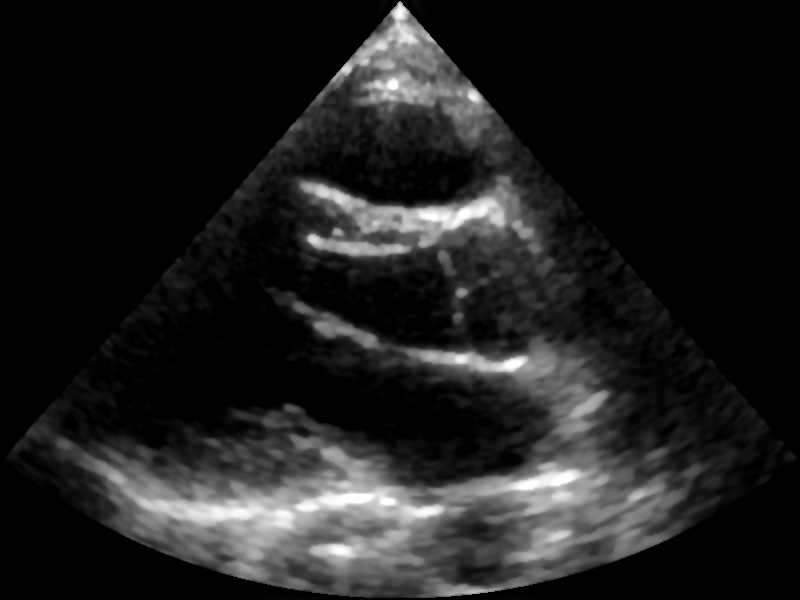
\includegraphics[width=\textwidth]{figures/cardiac1_lpndsf.png}};
      \spy on (0.05, 0.05) in node [redwindow, anchor=north] at ($(figA.south)$);
    \end{tikzpicture}
    \caption{LPNDSF}
  \end{subfigure}%
  \begin{subfigure}[b]{0.15\textwidth}
    \begin{tikzpicture}[
        spy using outlines={%
          rectangle,magnification=3,size=\textwidth,
          every spy on node/.append style={transparentwindow}
        }
      ]
      \node (figA) at (0.0,0.0) {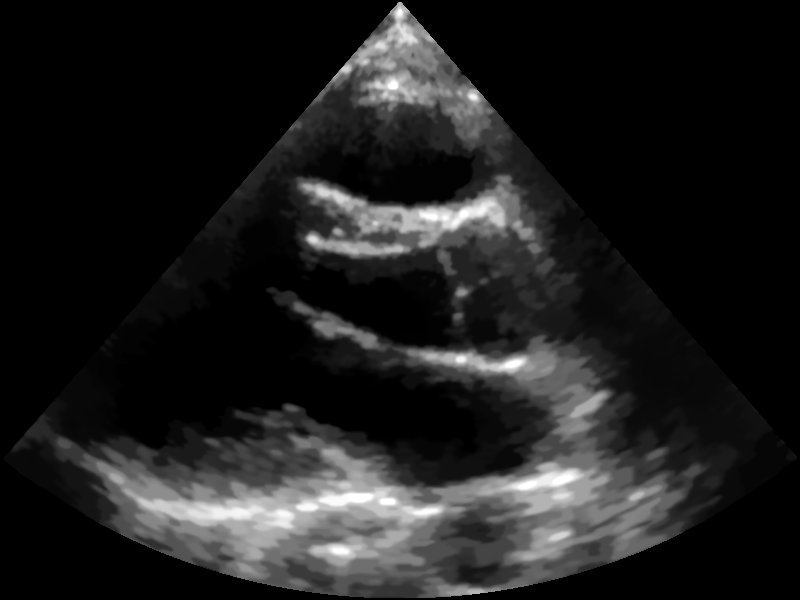
\includegraphics[width=\textwidth]{figures/cardiac1_mnlm.png}};
      \spy on (0.05, 0.05) in node [redwindow, anchor=north] at ($(figA.south)$);
    \end{tikzpicture}
    \caption{MNLM}
  \end{subfigure}%
  \begin{subfigure}[b]{0.15\textwidth}
    \begin{tikzpicture}[
        spy using outlines={%
          rectangle,magnification=3,size=\textwidth,
          every spy on node/.append style={transparentwindow}
        }
      ]
      \node (figA) at (0.0,0.0) {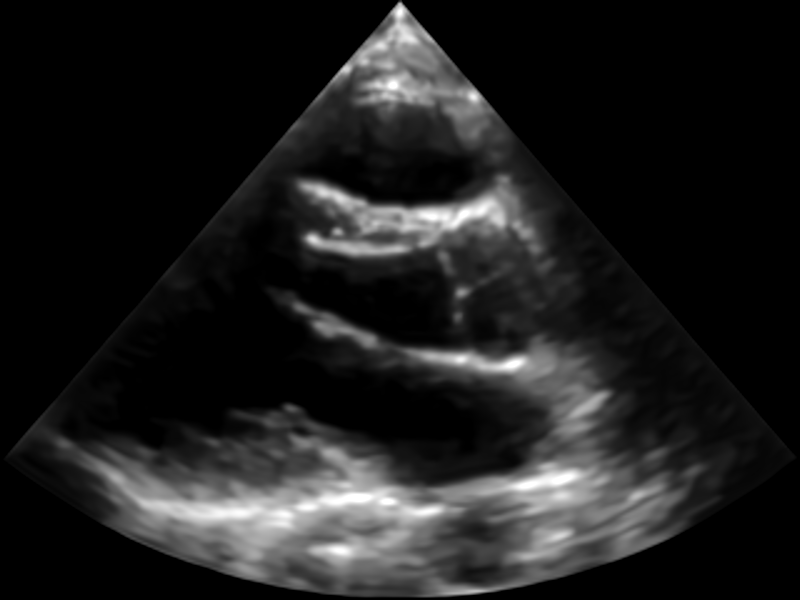
\includegraphics[width=\textwidth]{figures/cardiac1_nllr.png}};
      \spy on (0.05, 0.05) in node [redwindow, anchor=north] at ($(figA.south)$);
    \end{tikzpicture}
    \caption{NLLR}
  \end{subfigure}%
  \begin{subfigure}[b]{0.15\textwidth}
    \begin{tikzpicture}[
        spy using outlines={%
          rectangle,magnification=3,size=\textwidth,
          every spy on node/.append style={transparentwindow}
        }
      ]
      \node (figA) at (0.0,0.0) {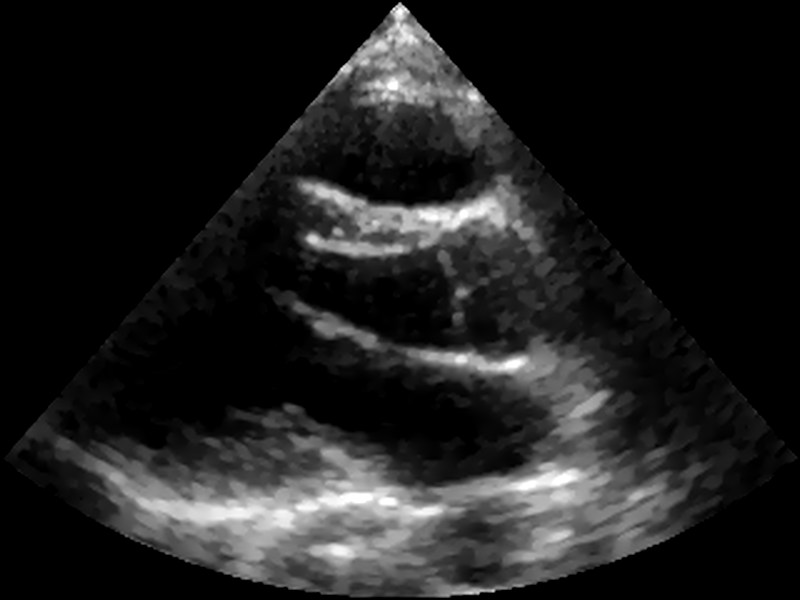
\includegraphics[width=\textwidth]{figures/cardiac1_pfdtv.png}};
      \spy on (0.05, 0.05) in node [redwindow, anchor=north] at ($(figA.south)$);
    \end{tikzpicture}
    \caption{PFDTV}
  \end{subfigure}\\
  %% \begin{subfigure}[b]{0.15\textwidth}
  %%   \begin{tikzpicture}[
  %%       spy using outlines={%
  %%         rectangle,magnification=3,size=\textwidth,
  %%         every spy on node/.append style={transparentwindow}
  %%       }
  %%     ]
  %%     \node (figA) at (0.0,0.0) {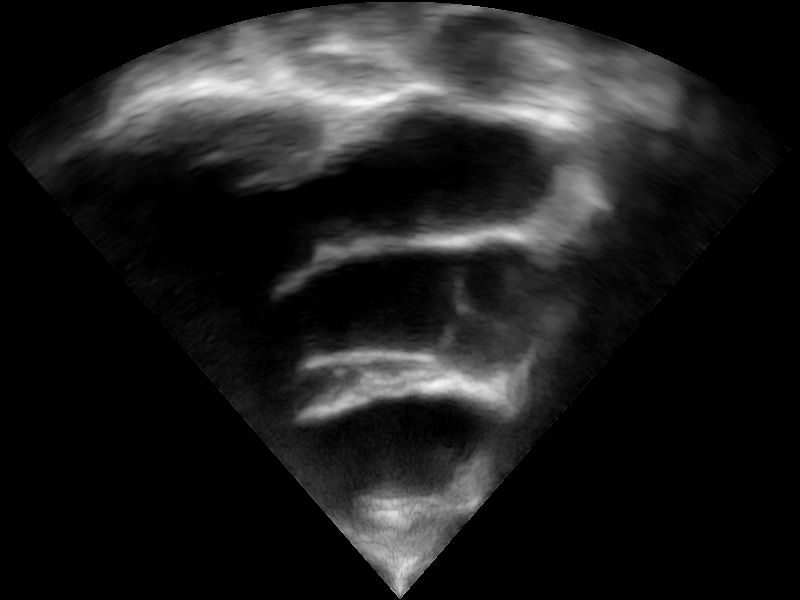
\includegraphics[width=\textwidth, trim={4cm 4cm 4cm 0cm}, clip]{figures/cardiac1_clpdQ.png}};
  %%     \spy on (0.05, 0.05) in node [redwindow, anchor=north] at ($(figA.south)$);
  %%   \end{tikzpicture}
  %%   \caption{CLPD-SSNR}
  %% \end{subfigure}%
  \begin{subfigure}[b]{0.15\textwidth}
    \begin{tikzpicture}[
        spy using outlines={%
          rectangle,magnification=3,size=\textwidth,
          every spy on node/.append style={transparentwindow}
        }
      ]
      \node (figA) at (0.0,0.0) {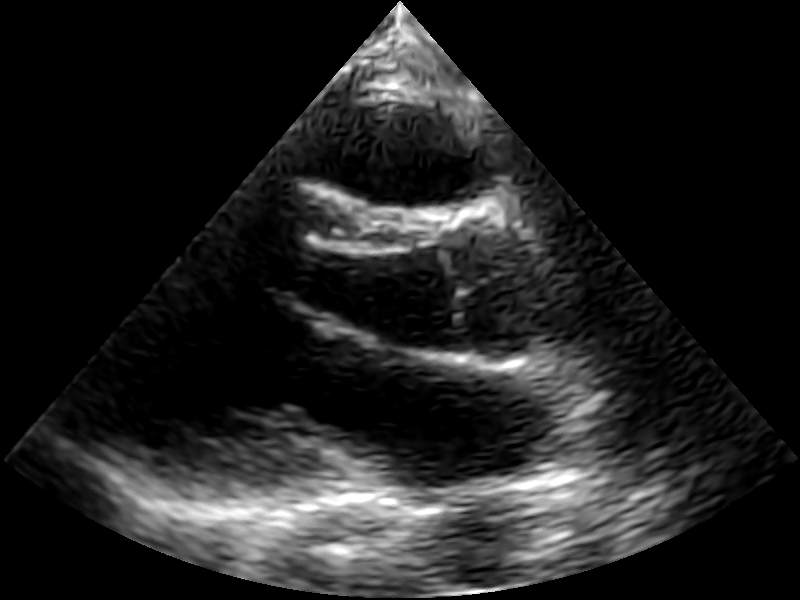
\includegraphics[width=\textwidth]{figures/cardiac1_clpda.png}};
      \spy on (0.05, 0.05) in node [redwindow, anchor=north] at ($(figA.south)$);
    \end{tikzpicture}
    \caption{CLPD-A}
  \end{subfigure}%
  \begin{subfigure}[b]{0.15\textwidth}
    \begin{tikzpicture}[
        spy using outlines={%
          rectangle,magnification=3,size=\textwidth,
          every spy on node/.append style={transparentwindow}
        }
      ]
      \node (figA) at (0.0,0.0) {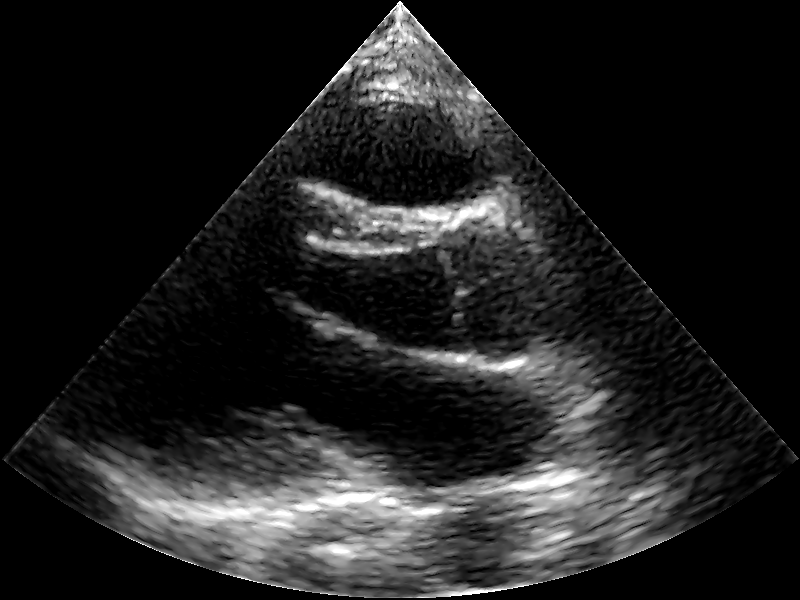
\includegraphics[width=\textwidth]{figures/cardiac1_clpdb.png}};
      \spy on (0.05, 0.05) in node [redwindow, anchor=north] at ($(figA.south)$);
    \end{tikzpicture}
    \caption{CLPD-B}
  \end{subfigure}%
  \begin{subfigure}[b]{0.15\textwidth}
    \begin{tikzpicture}[
        spy using outlines={%
          rectangle,magnification=3,size=\textwidth,
          every spy on node/.append style={transparentwindow}
        }
      ]
      \node (figA) at (0.0,0.0) {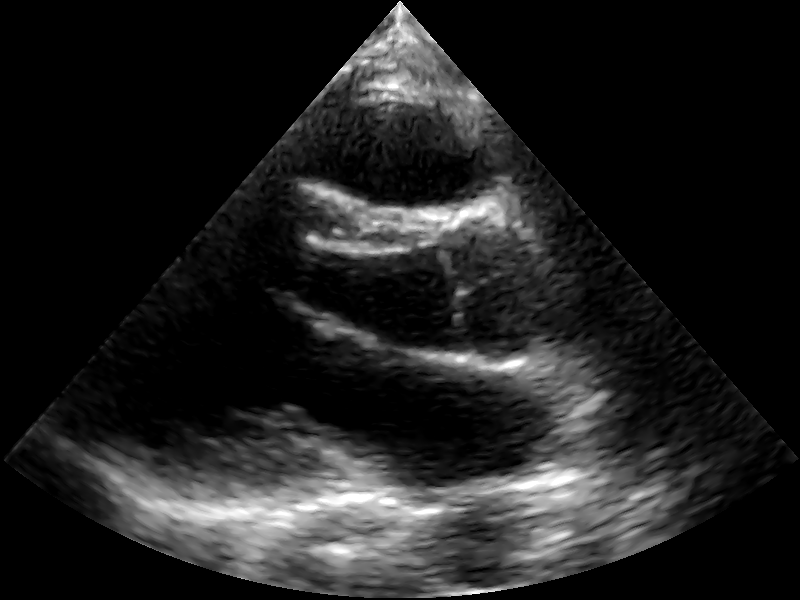
\includegraphics[width=\textwidth]{figures/cardiac1_clpdc.png}};
      \spy on (0.05, 0.05) in node [redwindow, anchor=north] at ($(figA.south)$);
    \end{tikzpicture}
    \caption{CLPD-C}
  \end{subfigure}%
  \begin{subfigure}[b]{0.15\textwidth}
    \begin{tikzpicture}[
        spy using outlines={%
          rectangle,magnification=3,size=\textwidth,
          every spy on node/.append style={transparentwindow}
        }
      ]
      \node (figA) at (0.0,0.0) {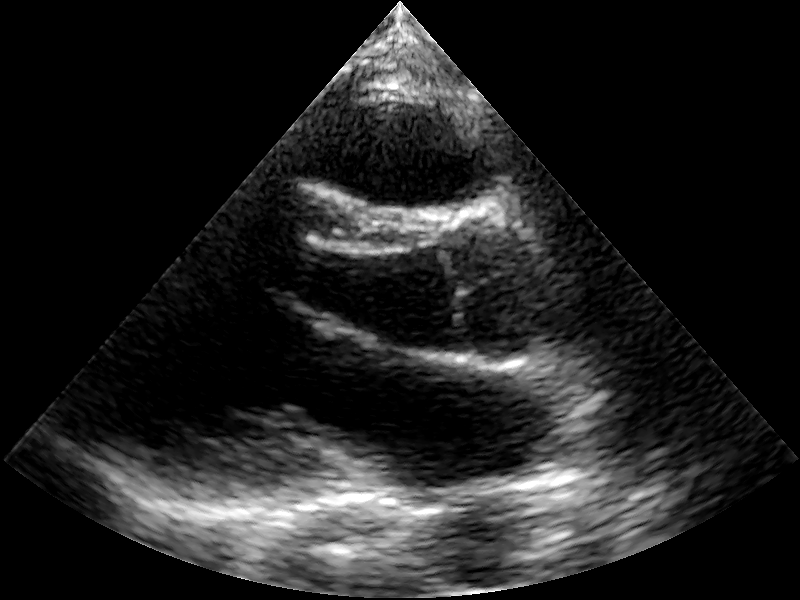
\includegraphics[width=\textwidth]{figures/cardiac1_clpdd.png}};
      \spy on (0.05, 0.05) in node [redwindow, anchor=north] at ($(figA.south)$);
    \end{tikzpicture}
    \caption{CLPD-D}
  \end{subfigure}%
  \begin{subfigure}[b]{0.15\textwidth}
    \begin{tikzpicture}[
        spy using outlines={%
          rectangle,magnification=3,size=\textwidth,
          every spy on node/.append style={redwindow}
        }
      ]
      \node (figA) at (0.0,0.0) {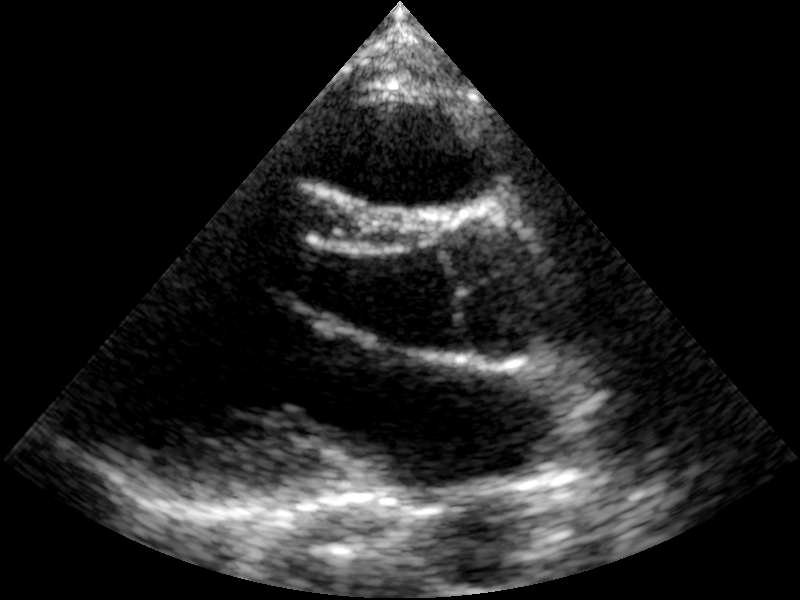
\includegraphics[width=\textwidth]{figures/cardiac1.png}};
      \spy on (0.05, 0.05) in node [redwindow, anchor=north] at ($(figA.south)$);
    \end{tikzpicture}
    \caption{Original}
  \end{subfigure}
  \caption{Results on echocardiography parasternal long-axis view.}\label{fig:cardiac1}
  \vspace{-0.1in}
\end{figure*}

%%% Local Variables:
%%% TeX-master: "master"
%%% End:

%
\subsubsection{Quantitative Results}
Quantitative results are shown in~\cref{table:liver1}.
We can see that the SSNR values obtained using the CLPDs are overall worse than the baselines except for CLPD-SSNR, which is natural since it was explicitly tuned to obtain a high SSNR.
This shows that, while it is possible to obtain a high SSNR with the CLPD, none of the sonographers preferred a high SSNR.
Instead, they preferred to preserve some level of speckle noise.
In contrast, all of the baselines except for ADMSS resulted in higher SSNR.
In particular, MNLM obtains the highest level of SSNR, which demonstrates that non-local means methods are excellent at removing speckle (which is, unfortunately, not always desirable).

Meanwhile, when looking at other metrics than the SSNR, the results look quite different.
The CLPDs obtained both high SSIM and high \(S_3\) overall.
Only ADMSS obtained a high SSIM, which is natural since it only selectively smooths pixels in the background.
CLPDs, on the other hand, all resulted in high levels of SSIMs, which shows that sonographers strongly prefer ``natural-looking'' images that do not deviate from the original image.

Lastly, when looking at the \(S_3\) metric, we can see that all CLPDs obtained high values.
This shows that the CLPD is capable of conserving sharpness and that sonographers strongly prefer sharp-looking images.
Indeed, most of the participating sonographers explicitly stated that they ``do not want to trade sharpness for less speckle'', a sentiment reflected by our results.
For this reason, the clinical value of NLLR is limited even though it is very good at reinforcing structures and reducing speckle.
%it results in significantly blurry images both qualitatively and quantitatively (according to \(S_3\)), which limits its clinical value.

\begin{table}
  \centering
  \caption{Quantatitive Results on Echocardiographic Apical 4-Chamber View}\label{table:cardiac3}
  \setlength{\tabcolsep}{3pt}
  \begin{threeparttable}
  \begin{tabular}{llrrrrr}
    \toprule
    & \multicolumn{1}{c}{\textbf{Algorithm}}
    & \multicolumn{1}{c}{\textbf{gCNR}}
    & \multicolumn{1}{c}{\textbf{CNR}}
    & \multicolumn{1}{c}{\textbf{SNR}}
    & \multicolumn{1}{c}{\textbf{SSIM}}
    & \multicolumn{1}{c}{\(\mathbf{S_{3}}\)}\\
    & \multicolumn{1}{c}{}
    & \multicolumn{1}{c}{}
    & \texttt{[dB]}
    & \texttt{[dB]}
    & \multicolumn{1}{c}{}
    & \multicolumn{1}{c}{} \\\midrule
    \multirow{6}{*}{Baselines}
    & OSRAD  & 0.490          & -1.62          & 4.51          & 0.891          & 0.500 \\
    & ADMSS  & 0.467          & -1.67          & 4.33          & \textbf{0.967} & 0.204 \\
    & LPNDSF & 0.473          & -1.67          & 4.39          & 0.868          & 0.458 \\
    & MNLM   & \textbf{0.534} & \textbf{-1.61} & 4.42          & 0.918          & 0.414 \\
    & NLLR   & \textbf{0.501} & \textbf{-1.60} & 4.61          & 0.857          & 0.042\\
    & PFDTV  & 0.480          & -1.65          & 4.49          & 0.865          & 0.155 \\  \cdashlinelr{1-7}
    \multirow{4}{*}{This work}
    & CLPD-A & 0.484          & -1.64          & \textbf{4.64} & \textbf{0.957} & \textbf{0.858} \\
    & CLPD-B & \textbf{0.496} & \textbf{-1.55} & \textbf{4.69} & \textbf{0.949} & \textbf{0.685} \\
    & CLPD-E & 0.476          & -1.63          & \textbf{4.61} & \textbf{0.961} & \textbf{0.507} \\
    & CLPD-F & \textbf{0.507} & \textbf{-1.50} & \textbf{4.79} & 0.920          & \textbf{0.705} \\\bottomrule
  \end{tabular}
  \begin{tablenotes}
    \item[*] The performance of the top 4 algorithms for each metric is shown in boldface.
  \end{tablenotes}
  \end{threeparttable}
  \vspace{-0.15in}
\end{table}
%
\subsection{Results on Echocardiographic Apical 4-Chamber View}\label{section:fourchamber}
%We now present results on a sequence of echocardiographic 4-chamber view images.

\subsubsection{Qualitative Results}
A representative frame processed by each method is shown in~\cref{fig:cardiac3}.
Similarly with the liver image, CLPD-A to CLPD-F turned out to be the least blurry.
Unlike the liver image, however, some of the expert tuned CLPDs showed substantial speckle reduction.
For example, the myocardium processed by CLPD-F shows the least speckle among all methods.
Despite the aggressive smoothing, it does not result in blurry images such as NLLR.
This shows the sharpness-preserving capability of our CLPD.

In addition, CLPDs resulted in smooth endocardium borders compared to the baselines, demonstrating its structure-enhancing capability.
In contrast, other methods were unable to fix the structural damages caused by speckle, and resulted in jiggly endocardium borders.
Although NLLR results in the best structural enhancement, the resulting blurriness shadows its benefits.

Meanwhile, CLPD-A can be seen emphasizing fine details.
The cardiologist (A) who tuned CLPD-A expressed his preference towards fine details such as papillary muscles.
On the other hand, sonographers stated that they focused on improving the contrast.
%Thus, some of the preferential variation in this case comes from the difference between the clinical focus of sonographers and cardiologists.
This clearly shows the preferential variation between experts on the same task.

Overall, we can see that the CLPD configurations tuned on the echocardiographic apical 4-chamber view are qualitatively different from those tuned on the liver costal view.
Our results points to the fact that image enhancement methods need to be tuned, not only to each clinical task but also to each individual.

\subsubsection{Quantitative Results}
%We now discuss the quantitative results on the echocardiographic 4-chamber image.

For echocardiographic images, recognizing different anatomical structures and their boundaries is an important clinic task.
Therefore, speckle reduction and contrast enhancement is more relevant, as reflected by the results in~\cref{table:cardiac3}.
All CLPD settings showed the highest SNR on the myocardium.
In terms of contrast, sonographers B and F showed a preference towards high gCNR and CNR.
However, CLPDs again unanimously achieved high SSIM and \(S_3\).

Among the considered baselines, MNLM and NLLR achieves a higher contrast, which is expected since both methods are known to be good at removing speckle.
However, they both result in low sharpness, while NLLR results in an unbelievably low \(S_3\) value.
Meanwhile, except for NLLR, all methods do not achieve a high SNR.
Although this is natural with ADMSS since it avoids reducing speckle on structural regions, the low SNR of MNLM is counter-intuitive.
From visual inspection, this seems to result from the inability of MNLM and other methods to improve the homogeneity of similar anatomical regions.
NLLR and CLPDs, on the other hand, are capable of improving the structural homogeneity.
This shows the importance of structural enhancement for echocardiographic images, which CLPDs achieves.

\subsection{Results on Echocardiographic Parasternal Long-Axis View}
Finally, we present qualitative results on an echocardiographic parasternal long-axis view sequence.
The parasternal long-axis view has many clinically relevant fine details, such as the mitral and aortic valves.
These fine details, however, are difficult to differentiate from speckle and clutter.

The results are shown in~\cref{fig:cardiac3}.
Unlike the echocardiographic apical 4-chamber view, all CLPDs amplify fine details regardless of speckle and clutter.
Flow-like artifacts resulting from aggressive coherence enhancement are clearly visible near the aortic valve.
As a result, the edges of the interventricular septum are enhanced.

%%% Local Variables:
%%% TeX-master: "master"
%%% End:
